%%%%%%%%%%%%%%%%%%%%%%%%%%%%%%%%%%%%%%%%%%
%Copyright (C) 2018-2020 YuZJ.
%使用CC-BY-NC-SA授权。一份完整版本的许可证已位于附录。这个版本原始作者YuZJ,
%邮箱theafamily@126.com(最后连接于2019年06月20日17:32:17)。
%%%%%%%%%%%%%%%%%%%%%%%%%%%%%%%%%%%%%%%%%%
\part{使用视窗操作系统实现教学任务}
对于中国的用户来说,视窗操作系统恐怕是最熟悉的操作系统了。该系统自Windows 3.1在中国发布,并在Windows95面市后以其美观易用(和虚弱的版权保护)横扫中国国产操作系统。因此作为一个被广为接受的操作系统,学习它是十分重要的。\par
作为微软公司最新发布的操作系统,Windows10以其美观的界面,强大的可操作性与兼容性成为目前为止最好的Windows操作系统\footnote{当然,见仁见智。微软的竞争对手比如说GNU就不这么认为。参考【微软公司的软件是恶意软件】\url{http://www.gnu.org/proprietary/malware-microsoft.html}(最后连接于2019年06月20日17:35:43)}。它还包括最新的IIS \footnote{Internet Information Service,互联网信息服务。IIS是一种Web服务组件。内含的Web服务器、FTP服务器、NNTP服务器和SMTP服务器,分别用于网页浏览、文件传输、新闻服务和邮件发送等方面。它简化了在网络上发布信息的流程。\cite{iisinfo}}、SmartScreen筛选器\footnote{一个网络安全检查程序,会检查你浏览的网页和下载内容是否含毒。}及.Net Framework \footnote{.Net Framework:到目前为止你只需要知道以下内容就行了:对于Windows XP,你应该安装.Net Framework 4.0。对于Windows7,你至少应该安装.Net Framework 4.8。Windows10自带.Net Framework。}与.Net Core。\par 
版本上,我建议使用“专业版”而不是“家庭版”(设备自带激活除外),因为专业版提供了家庭版所不具有的管理功能(如组策略)。专业版已经可以胜任教学操作,不需要升级为专业工作站版。\par
安装32位还是64位?32位的CPU仅能安装32位操作系统,64位的CPU可安装两者。32位的操作系统仅能运行32位程序,而64位的操作系统可运行两者且效率更高。目前几乎所有市面上的CPU(如Intel Core i3/i5/i7 \nth{8} Gen)均为64位架构,且仅支持Windows10 64位和部分版本的GNU/Linux操作系统。AMD64(直译为由AMD公司推出的64位架构)与x86\_64(Intel在x86架构下开发的64位版本x86,简写x64)在这里不作区分。arm64为高通制造的64位处理器,一般仅仅安装在手机、平板电脑或其他轻薄本、二合一本上,不常见。此时你应该选择Windows10 arm64这个特殊的版本。很抱歉,ARM64目前还无法不使用其它手段(如模拟器)运行x64或AMD64应用程序,但它对Microsoft Store应用支持较好并且可以运行32位应用程序。按照Debian GNU/Linux的分类方法,x64架构被并到了AMD64。32位系统则被称为i386或i686。如果你从某些自由软件生产商处下载应用程序(如GNU Emacs),你就应该明白这点。当然国产CPU应视情况而定,如龙芯使用MIPS指令集,华为使用ARM,兆芯使用x64。\par
你可以在“我的电脑”(Windows7)或“此电脑”(Windows10)或上右击——属性,在“系统”栏目中能看到“系统类型”中是32位操作系统还是64位操作系统(比如说,对于x64位的操作系统你会发现“64位操作系统,基于x64处理器”)。
\section{安装}
要学习一个操作系统,你首先要安装它。下面以介绍了一些简单的方法。注意,为避免病毒侵入(以及安装时下载更新),安装时请断网。{\color{red}警告!即使使用微软提供的映像,第三方安装工具也可能会向计算机注入病毒或安装用户不需要的软件!因此请尽量不要使用非官方的工具来安装系统!}\par
我建议你在安装视窗操作系统时先备份磁盘上的数据(非系统盘直接复制,系统盘使用Ghost或dd命令),并参考电教员有关计算机上预装的操作系统的消息。为运行流畅,你需要至少150GB的空闲硬盘空间和8GB内存。
\subsection{法一:自Windows7及以上升级}
自Windows7及以上的操作系统(指Windows7,Windows8,Windows8.1及较旧版本的Windows10)升级是一个明智的决定。它能够保存你的大部分信息、文件及软件但不能在32位于64位之间自由切换。\par
首先你需要一个工具:Media Creation Tool。它可在【下载Windows10】\url{https://www.microsoft.com/zh-cn/software-download/windows10}(最后连接于2019年06月20日18:14:17)处被下载。之后以管理员权限运行它(为了实现这一步,你需要以“Administrator”账户登录,并右击该程序,选择“以管理员权限运行”)。将会弹出“适用的声明和许可条款”,请在{\color{red}仔细阅读}后选择“我接受许可条款”(当然你也可以选择退出安装,如果你不同意)并单击“下一步”,在“你想执行什么操作?”时单击“升级这台电脑”。之后将会下载Windows10并创建介质,真正的安装程序将从介质中启动。大部分随后的操作与法二相同,在此不再赘述。
\subsection{法二:使用安装光盘或USB设备引导安装}
对于希望更加自由地安装操作系统并有一定技术水平的人可以选择安装光盘或USB设备引导安装。安装镜像可在【下载 Windows10 光盘映像(ISO 文件)】\url{https://www.microsoft.com/zh-cn/software-download/windows10ISO}(最后连接于2019年06月20日18:14:17)得到或在Media Creation Tool中创建。\par
先介绍Rufus的基本使用。Rufus可以将可启动的光盘映像写入U盘。下载:官网【RUFUS】\url{https://rufus.ie/}(最后连接于2019年06月20日18:15:53)。首先在“设备”中选择你的u盘,引导选择“镜像文件”,再选择对应镜像。之后直接按“开始”,一路“确定”即可。Rufus还可用于烧录GNU/Linux镜像。Rufus的最新版本也支持下载Windows10。如果你没有光盘刻录机或DVD-R(W)光盘,你可以使用Rufus将一个iso文件写入u盘,或直接使用Media Creation Tool。
\begin{center}
	\includegraphics[scale=0.4]{pic/Rufus}	
\end{center} \par
现在你手头上应该有一张Windows10光盘(或U盘,下同)。现在请重启计算机,当主板画面出现时,按住“F12”。在随之出现的启动菜单中选择光盘驱动器。你将看到(仅限于同时具有32位与64位的映像。仅有其中一种架构的映像将会跳过这一步。)使用UEFI的机器还会有一个“Press any key to boot from CD/DVD”,此时你应该按回车键:
\begin{center}
	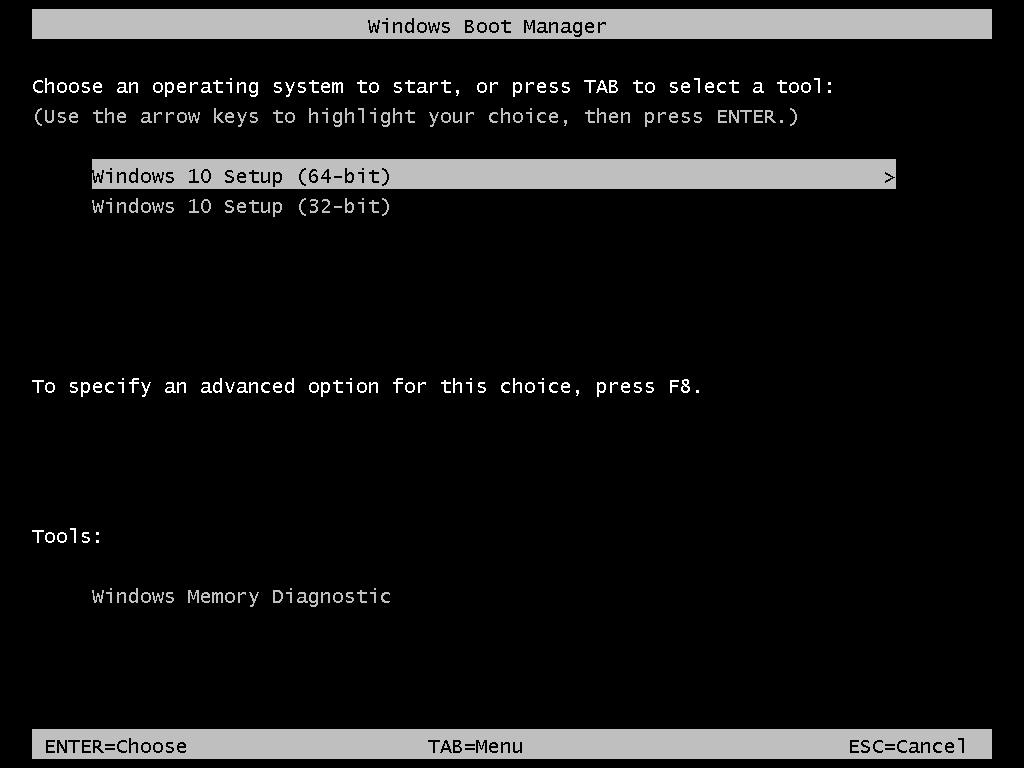
\includegraphics[scale=0.3]{pic/win10setup1}
\end{center} \par
现在请移动高亮条至你需要安装的架构(一般选择64位,下面以64位为例),并单击回车键。在“加载文件”(英文:Loading Files)与Windows徽标(有可能你会看到主板徽标)出现后,你将看到左图。这里你可以保持大部分设置不变(当然,喜欢使用五笔输入法的可以更改输入法为“微软五笔”)。单击“下一步”,在下一个对话框中单击“现在安装”。你将看到右图。
\begin{center}
	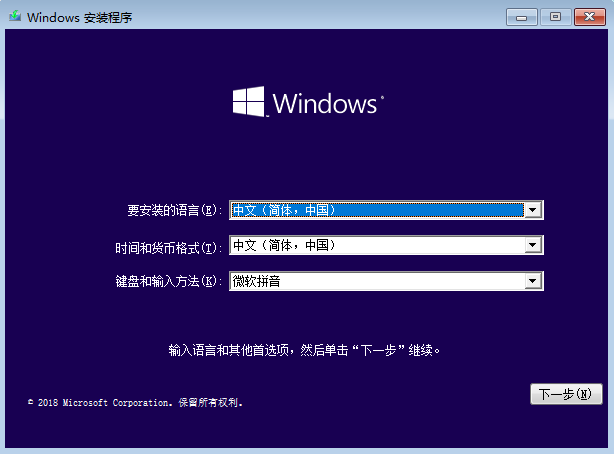
\includegraphics[scale=0.5]{pic/win10setup2}\\	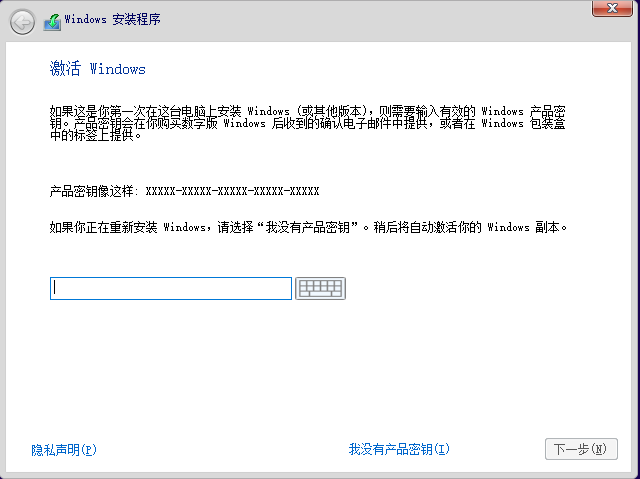
\includegraphics[scale=0.5]{pic/win10setup3}
\end{center} \par
此时如果你有序列号,请在这里输入它;如果你没有序列号(比如说,你的机器自带激活),请单击“我没有产品密钥”。随后会弹出“适用的声明和许可条款”,请在{\color{red}仔细阅读}后选择“我接受许可条款”并单击“下一步”。当然你也可以选择退出安装,如果你不同意。\par
之后选择安装类型。如果你只是需要升级,请单击“升级”。注意,此步仅限升级兼容的操作系统。如果兼容性检查失败或需要进行其它配置,请单击“自定义”。你将看到左图。下面以双硬盘空白安装为例(你的计算机也许只有一块硬盘)安装Windows10。如图,我们的机器目前有两块硬盘,我们需要在其中的一块硬盘上安装Windows操作系统(包括一个60GB的系统盘“System”与一个40GB的文件盘“Files”)选中“驱动器0 未分配的空间”,单击“新建”,你将看到右图。
\begin{center}
	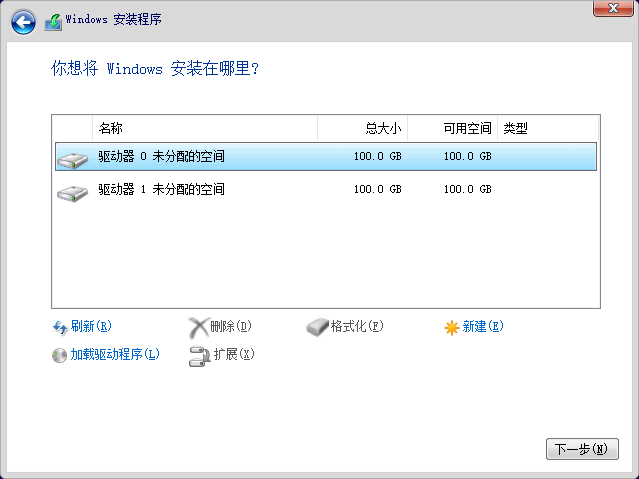
\includegraphics[scale=0.5]{pic/win10setup4}\\	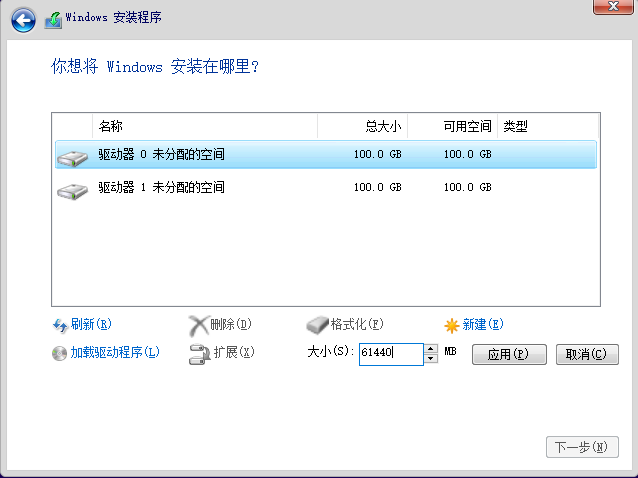
\includegraphics[scale=0.5]{pic/win10setup5}
\end{center} \par
输入系统盘大小\footnote{以61440MB(60GB)为例,其实你需要更大的系统盘。对于固态硬盘用户:你当然可以将整个固态硬盘作为系统盘。此时你只需选中那个驱动器并单击“确定”。},单击“应用”。在弹出的对话框选择“确定”。你会发现多出来了一个“系统保留”分区并且系统盘大小似乎改变了,不用管它。{\color{red}这里演示的是老型号机器:BIOS-Legacy的主板,设置使用主启动记录(MBR)的分区表格式安装。使用BIOS-UEFI安装过程大体相同,只是分区上多了“恢复”“系统分区”“MSR(保留)”“主分区”,你需要在“主分区”安装它。}。我又将剩余空间分了一个盘(对于另外一块硬盘,我们不需要管它。我们之后会用到的)。你见看到左图。选择驱动器0分区2--我的系统盘{\color{red}(注意!)},单击“下一步”,Windows就开始安装了。你将看到右图。
\begin{center}
	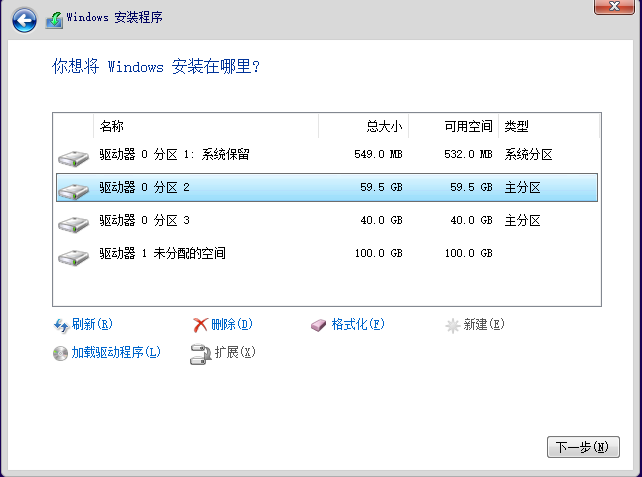
\includegraphics[scale=0.5]{pic/win10setup6}\\	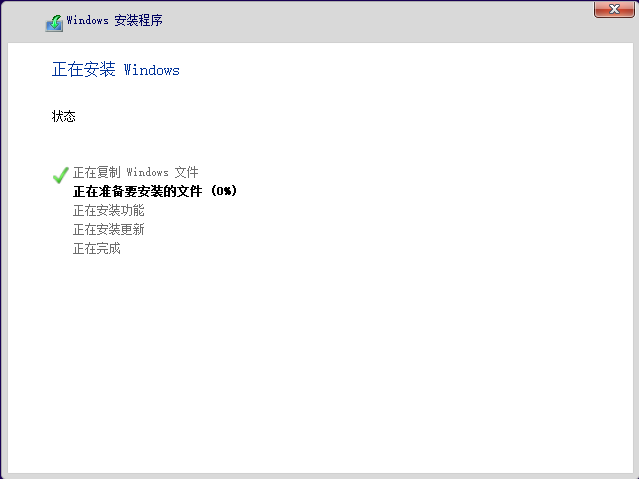
\includegraphics[scale=0.5]{pic/win10setup7}
\end{center} \par
安装完后将会重启。{\color{red},弹出光盘!}对于之后的操作,我认为Cortana会提示你的。关于账户:由于这台计算机为班内使用,请选择“脱机账户”。账户名一般写为“Administrator(即“管理员”。此次我写为SGComputers,密码为空)。安装完成后,你将看到:
\begin{center}
	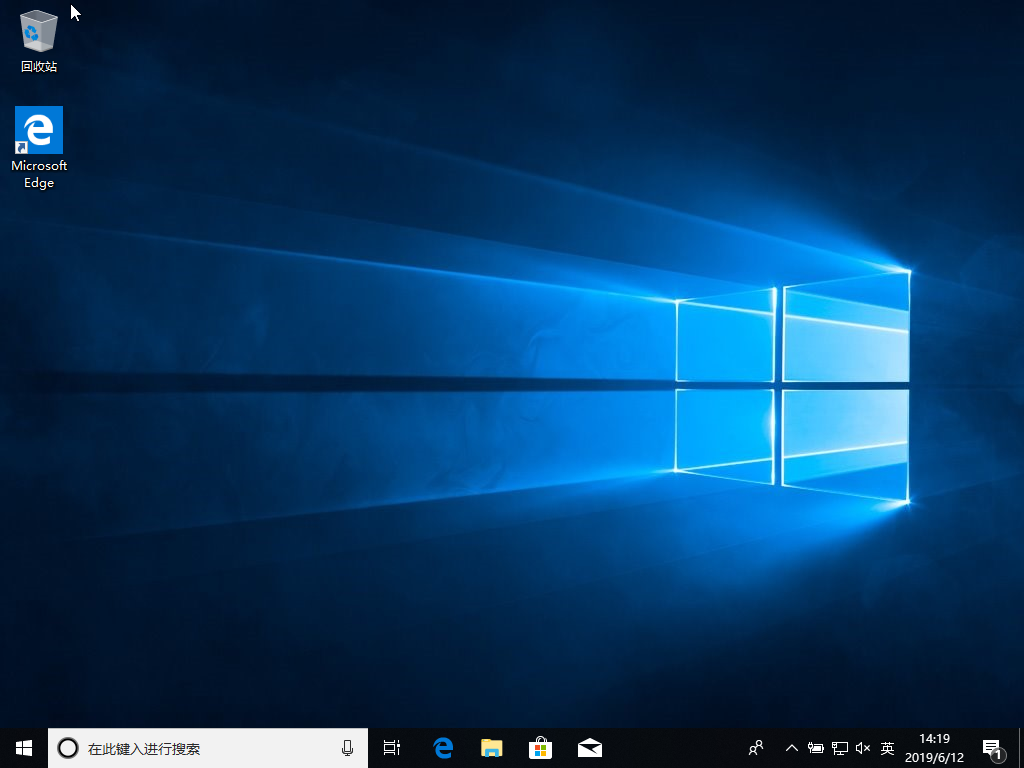
\includegraphics[scale=0.3]{pic/win10setup8}
\end{center}\par
现在你可以插上网线了。
\subsection{法三:基于磁盘映像的安装方法}
如果我们希望将一台计算机上的操作系统复制到另一台计算机或需要批量安装定制的操作系统,最好的方法是使用磁盘映像。该操作需要Windows PE(Ghost(.gho)及7z,wim,rar格式)或GNU/Linux(其他压缩格式或dd命令产生的磁盘映像)。不要试图在需要备份的Widows运行时运行任意一款磁盘备份软件。你需要等待它关机以后执行备份/还原。这里以Ghost映像为例。\par
首先请注意赛门铁克似乎已经放弃对个人用户的Ghost支持了。我在他们的官方网站上找不到对于个人的Ghost软件。下面使用的Ghost软件是从一个WinPE中提取的,版本号11.0.2.1573,SHA-256为42853A21787637FEFA5D9C6CB2CB8FD28E0AE36D8ABA776199AC033620D96467。以管理员权限运行它,你将得到:
\begin{center}
	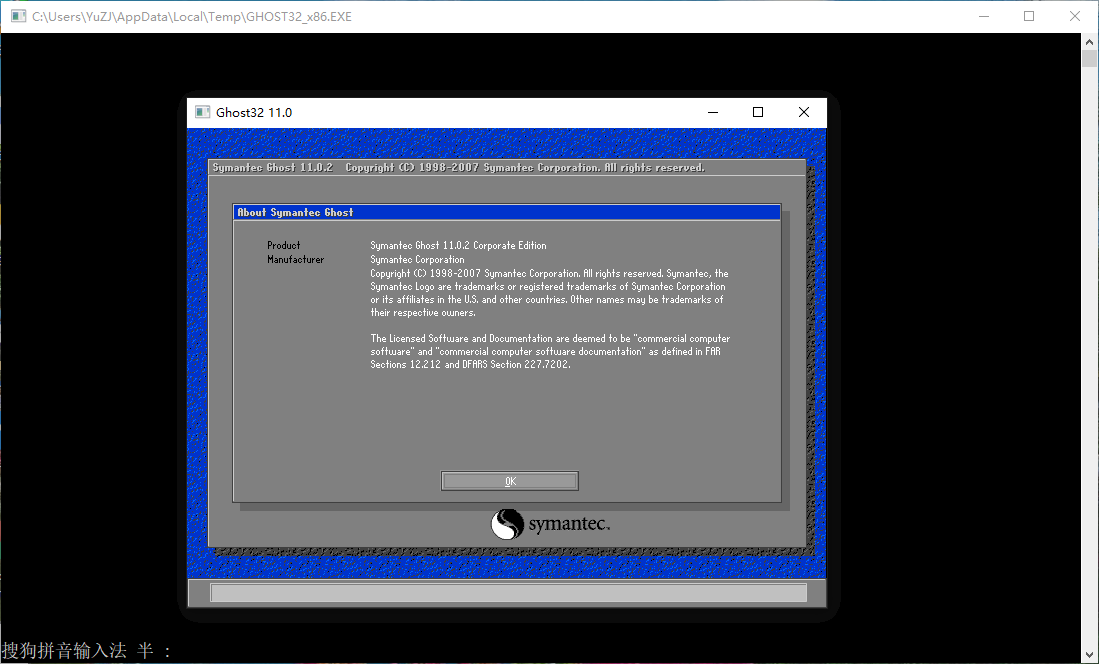
\includegraphics[scale=0.4]{pic/sg1}
\end{center}\par
单击“OK”,你将得到主界面:
\begin{center}
	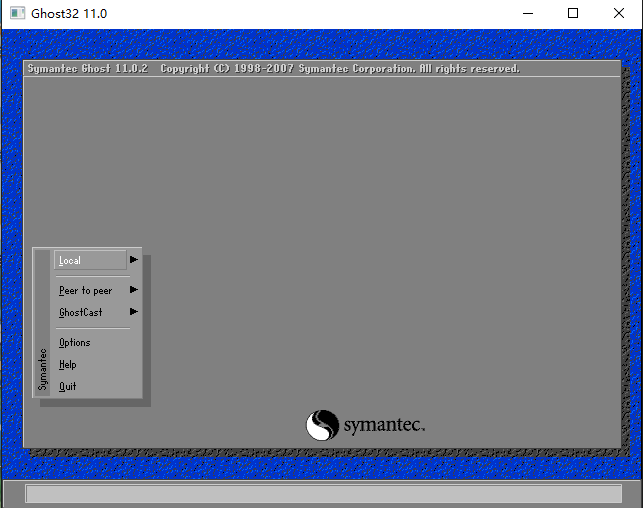
\includegraphics[scale=0.5]{pic/sg2}
\end{center}\par
现在假设我们需要备份Z盘,我们就应该在这个地方单击一下:
\begin{center}
	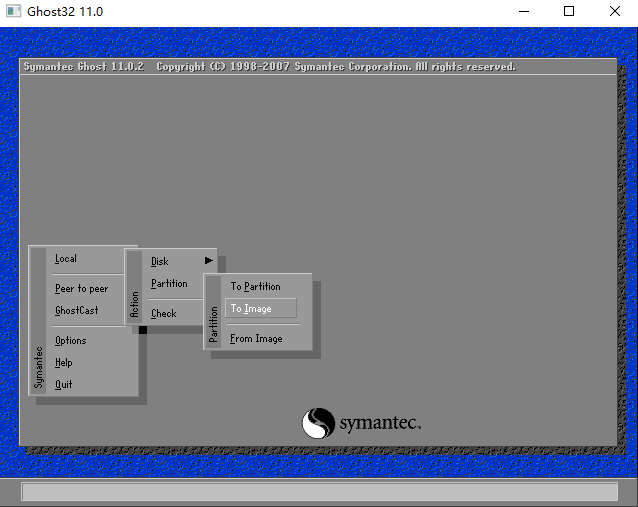
\includegraphics[scale=0.5]{pic/sg3}
\end{center}\par
选择设备和分区(这个可以根据硬盘生产商和容量鉴别):
\begin{center}
	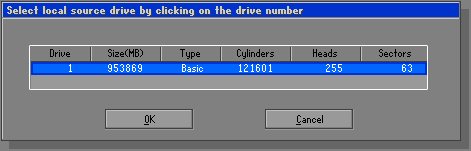
\includegraphics[scale=0.5]{pic/sg4}\\
	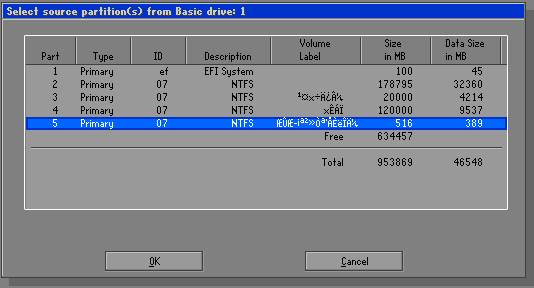
\includegraphics[scale=0.5]{pic/sg5}
\end{center}\par
选择保存位置:
\begin{center}
	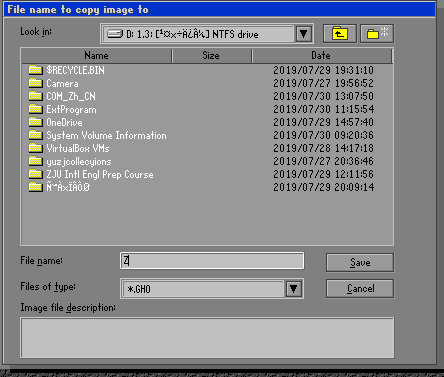
\includegraphics[scale=0.5]{pic/sg6}
\end{center}\par
是否压缩(这个按照自己的要求选择,压缩高耗时长):
\begin{center}
	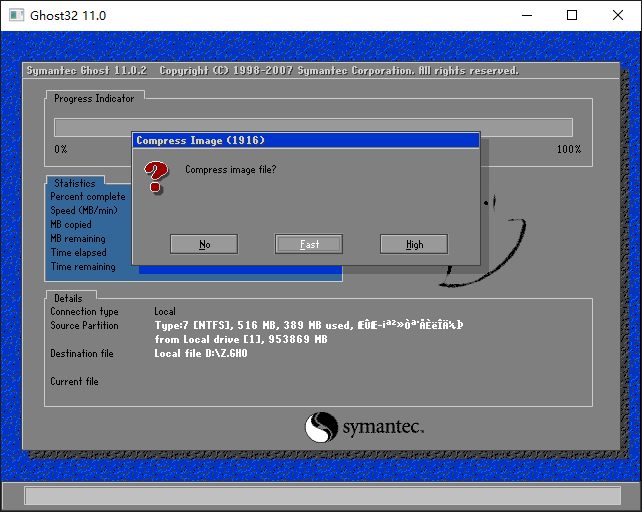
\includegraphics[scale=0.5]{pic/sg7}
\end{center}\par
再进行一次确认就开始操作:
\begin{center}
	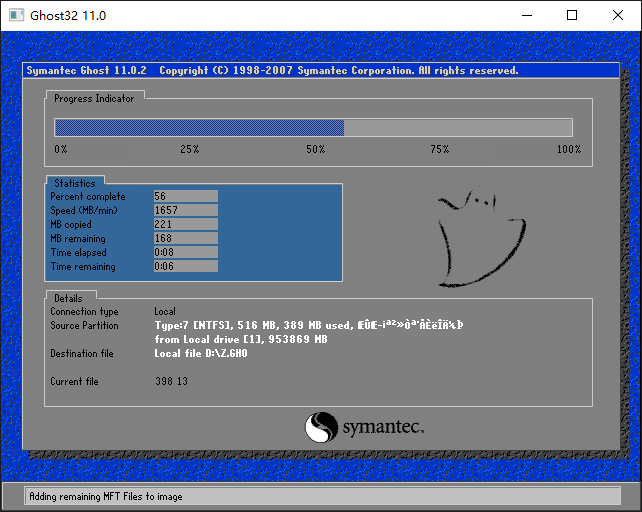
\includegraphics[scale=0.5]{pic/sg8}
\end{center}\par
从备份恢复操作类似。Ghost还提供了磁盘到磁盘、分区到分区等复制功能。注意,这个软件仅支持Windows分区,要修改GNU/Linux分区请使用dd命令。
\chapter{-开箱设置}
这一章节将介绍安装完Windows10操作系统后的“开箱设置(First Things First)”。包括:实现日常教学所需的软件,自动更新及常见的反病毒软件。关于Win10自带的OneDrive的使用将会在\pageref{sec:OneDrive}页的\ref{sec:OneDrive}章节讲到。\par
按照一般人的操作习惯,首先你需要在桌面上得到“此电脑”。找到“开始”菜单--设置--个性化(一个大方块)--主题(左边的长方形)--桌面图标设置(如图),选中“计算机”后单击“确定”。
\begin{center}
	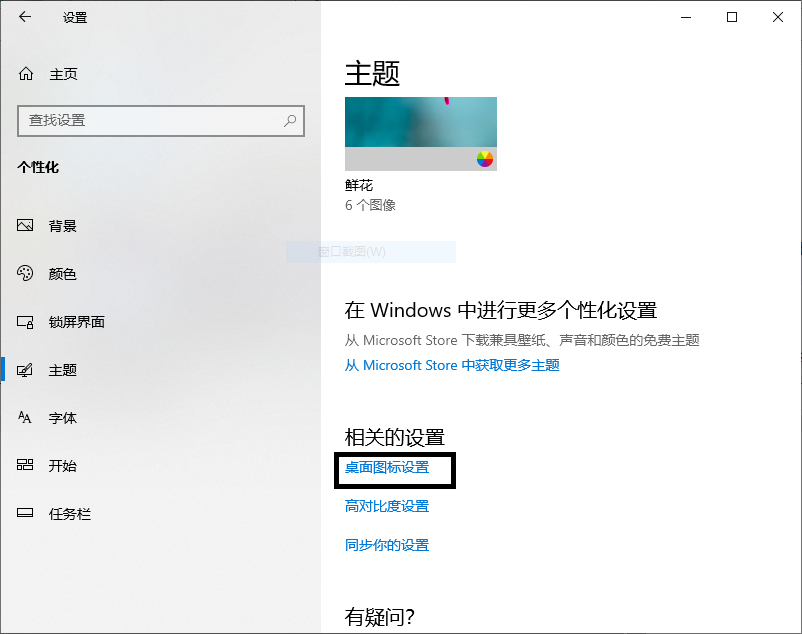
\includegraphics[scale=0.3]{pic/WinComp}
\end{center} 
\section{-基本概念及操作}
\subsection{屏幕(Screen)}
现在你已经安装好了Windows10操作系统。首先你需要知道什么是“屏幕”。我们将你在显示器上看到的部分称为“屏幕”。就像这样:
\begin{center}
	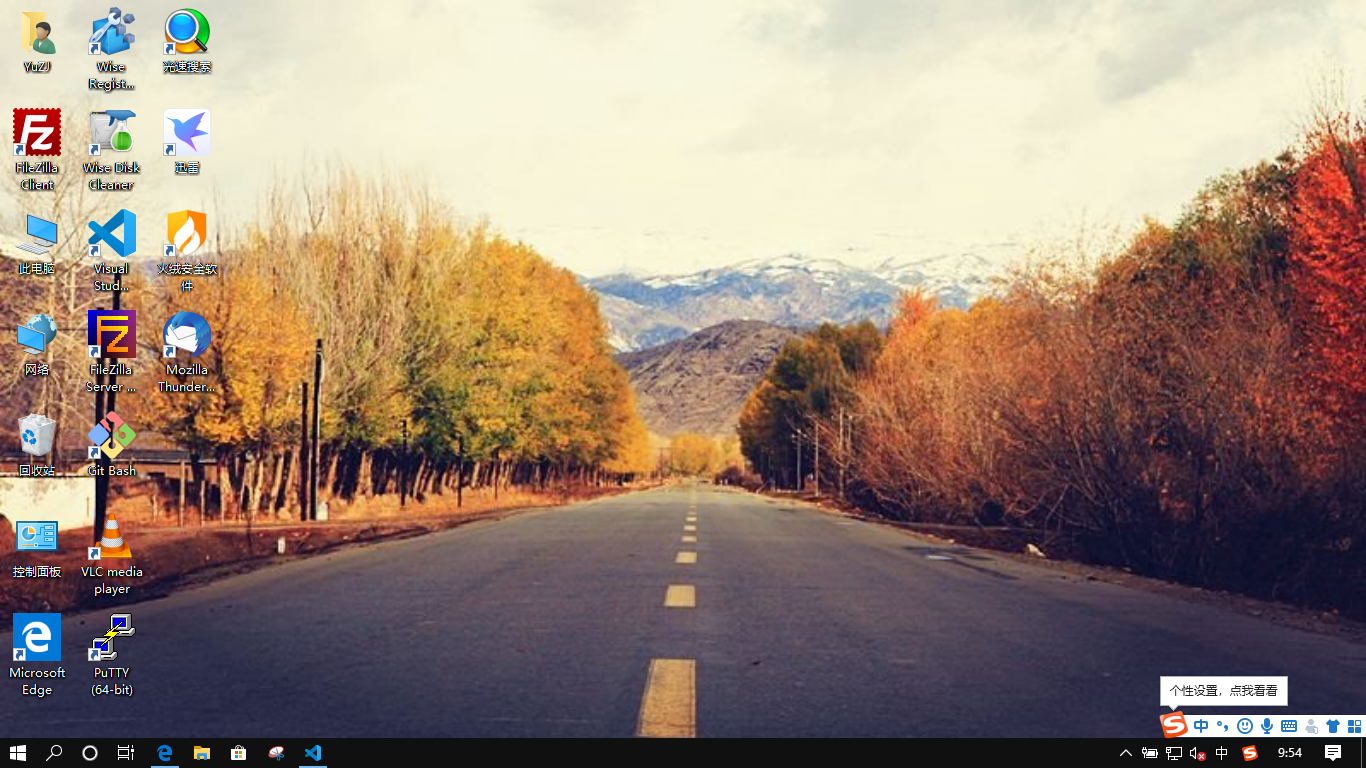
\includegraphics[scale=0.25]{pic/screen}
\end{center} \par
这就是一个“屏幕”。现在请观察一下线路连接。如果你使用的是教室内的带投影的台式计算机,你会发现由计算机上的VGA口连出了一条较粗的电缆到中央控制器的VGA口。另几条电缆由类似的接口连接到投影仪和显示器。这种情况下你会发现显示器上的图像与投影仪上的图像几乎是同步的。此时我们将其计算做一个屏幕。\par
如果你连接到多台显示器,你会得到几个屏幕?答案不一定相同。你可以进入“设置”-“显示”查看情况。你会发现“多显示器设置”菜单有多种选择——“复制”(就是指将主显示器上的图像复制到副显示器上面,常见的有两个显示器的柜台机就是这种构造)与“扩展”(相当于把副显示器与主显示器合二为一形成了一块较大的屏幕)。效果如下图所示。我们将第一种情况认定为1块屏幕,第二种两块。
\begin{center}
	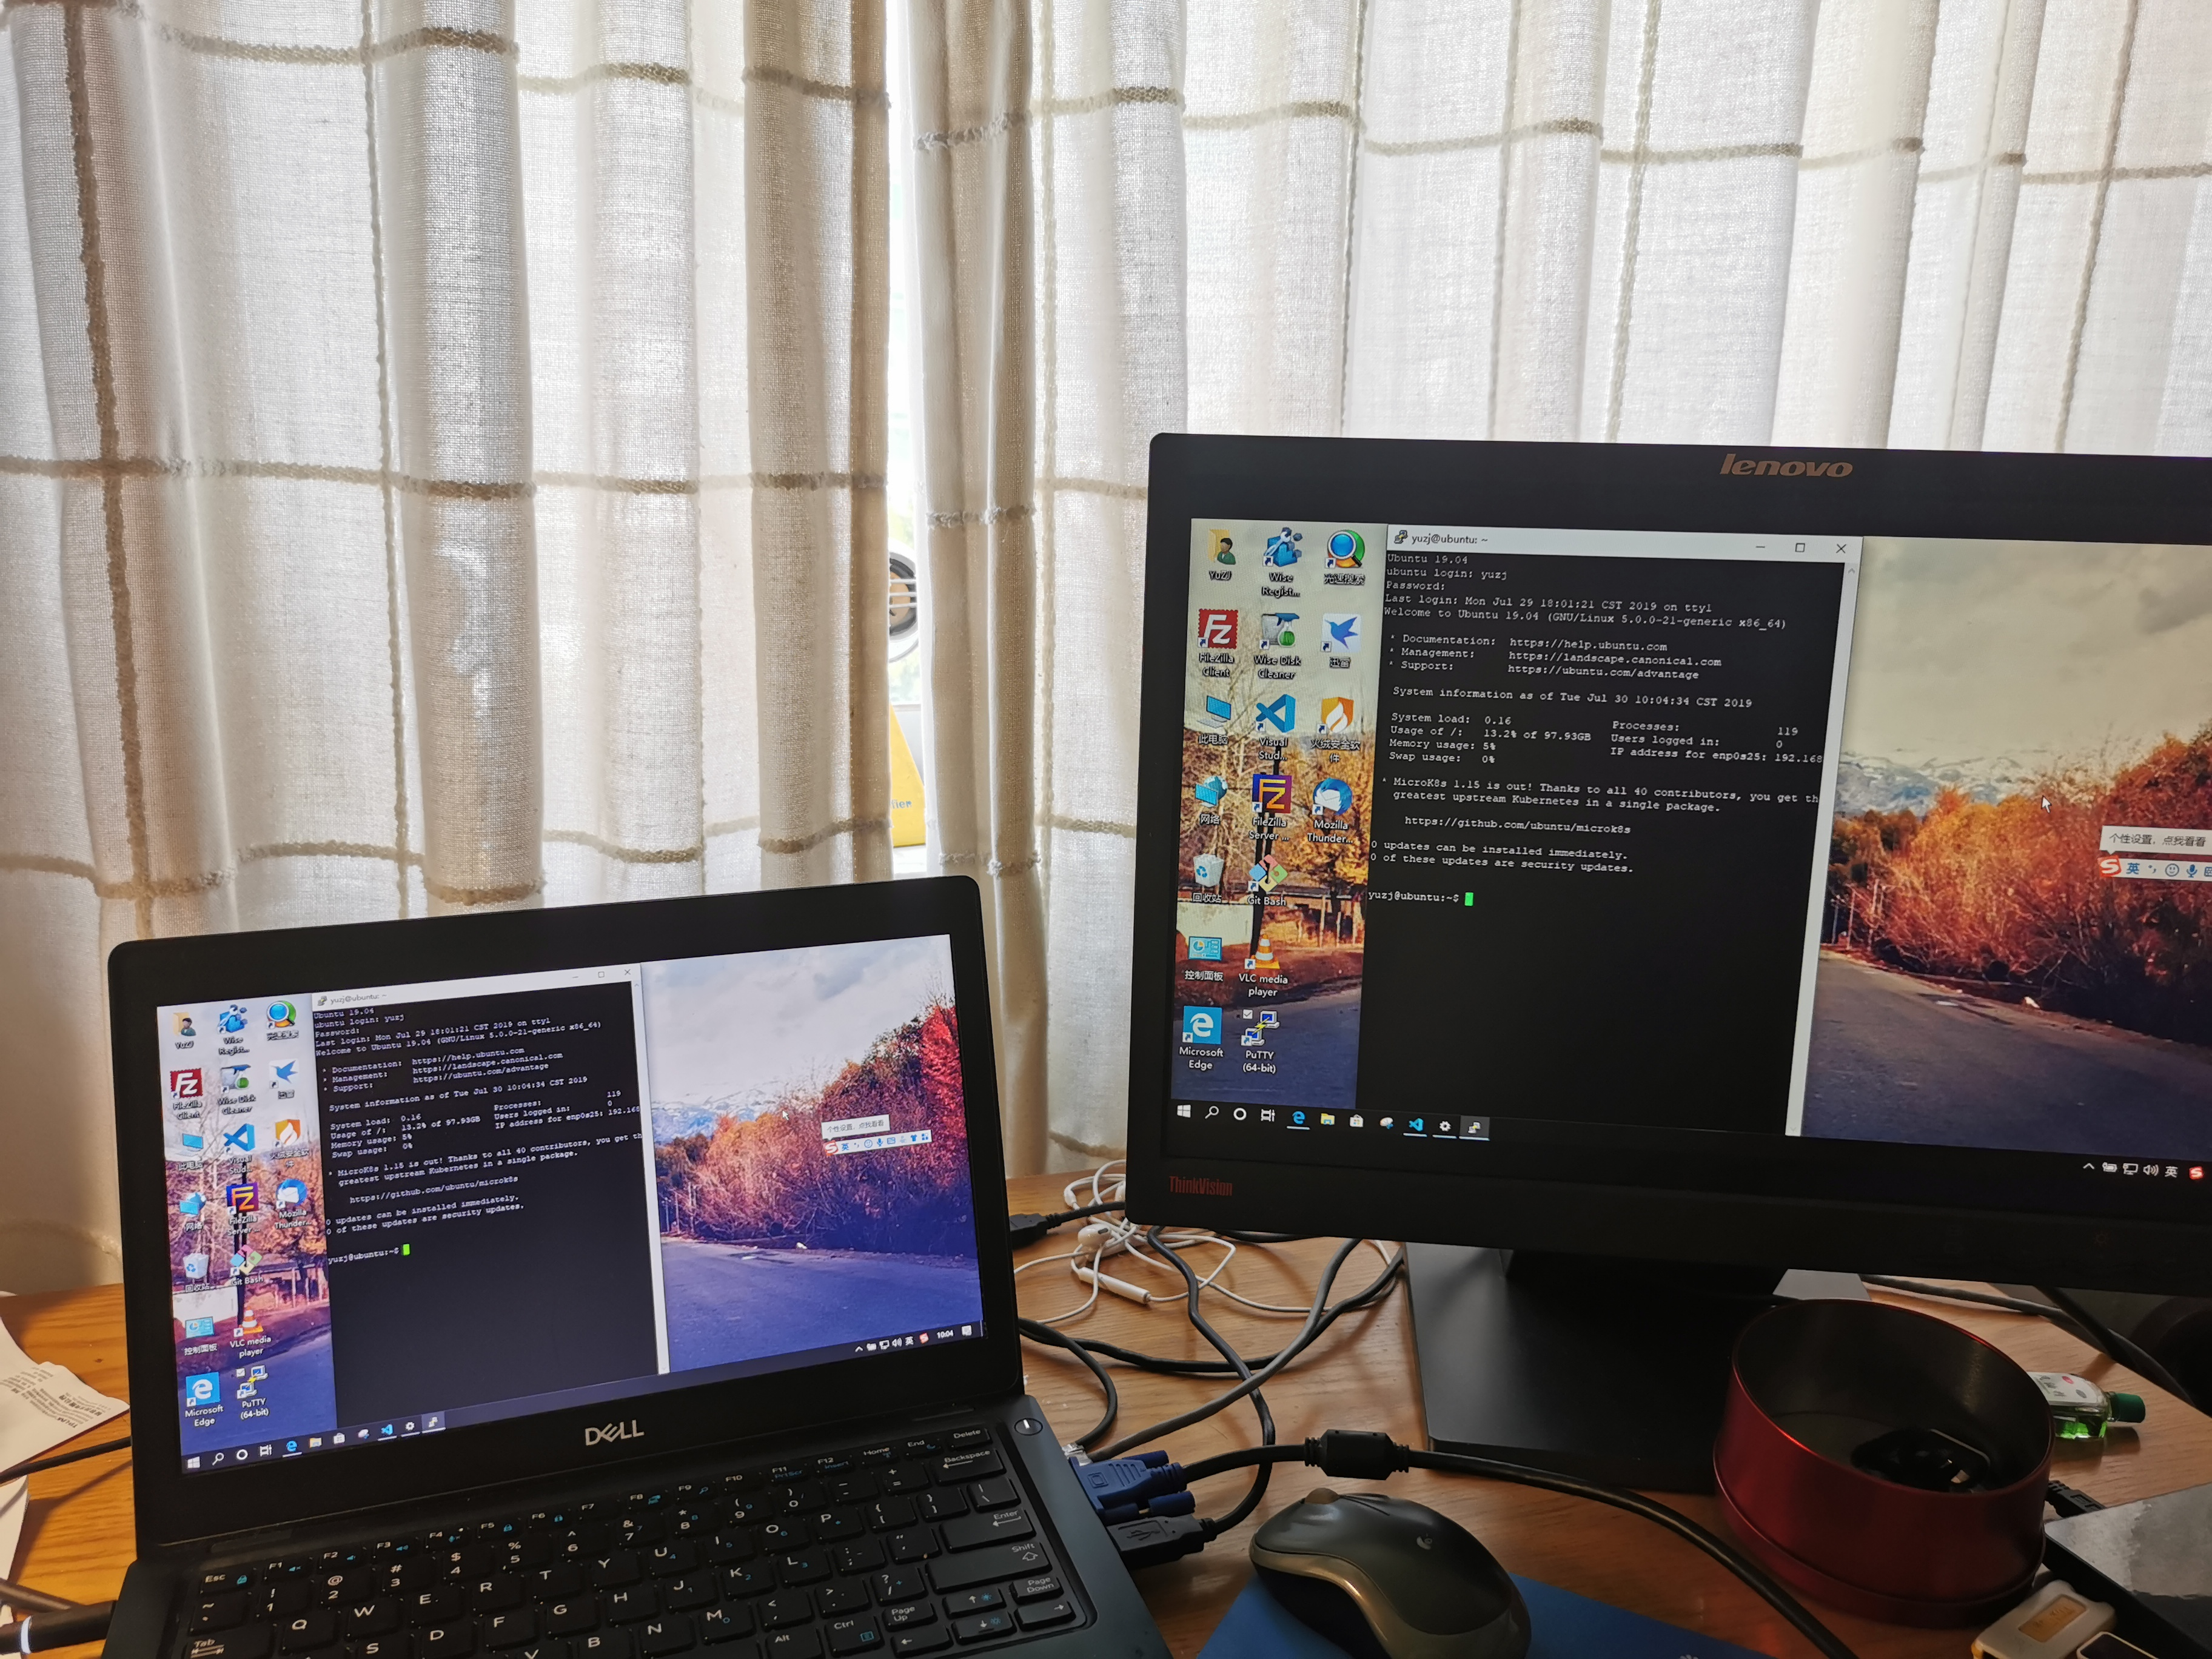
\includegraphics[scale=0.08]{pic/ScrCopy}\\
	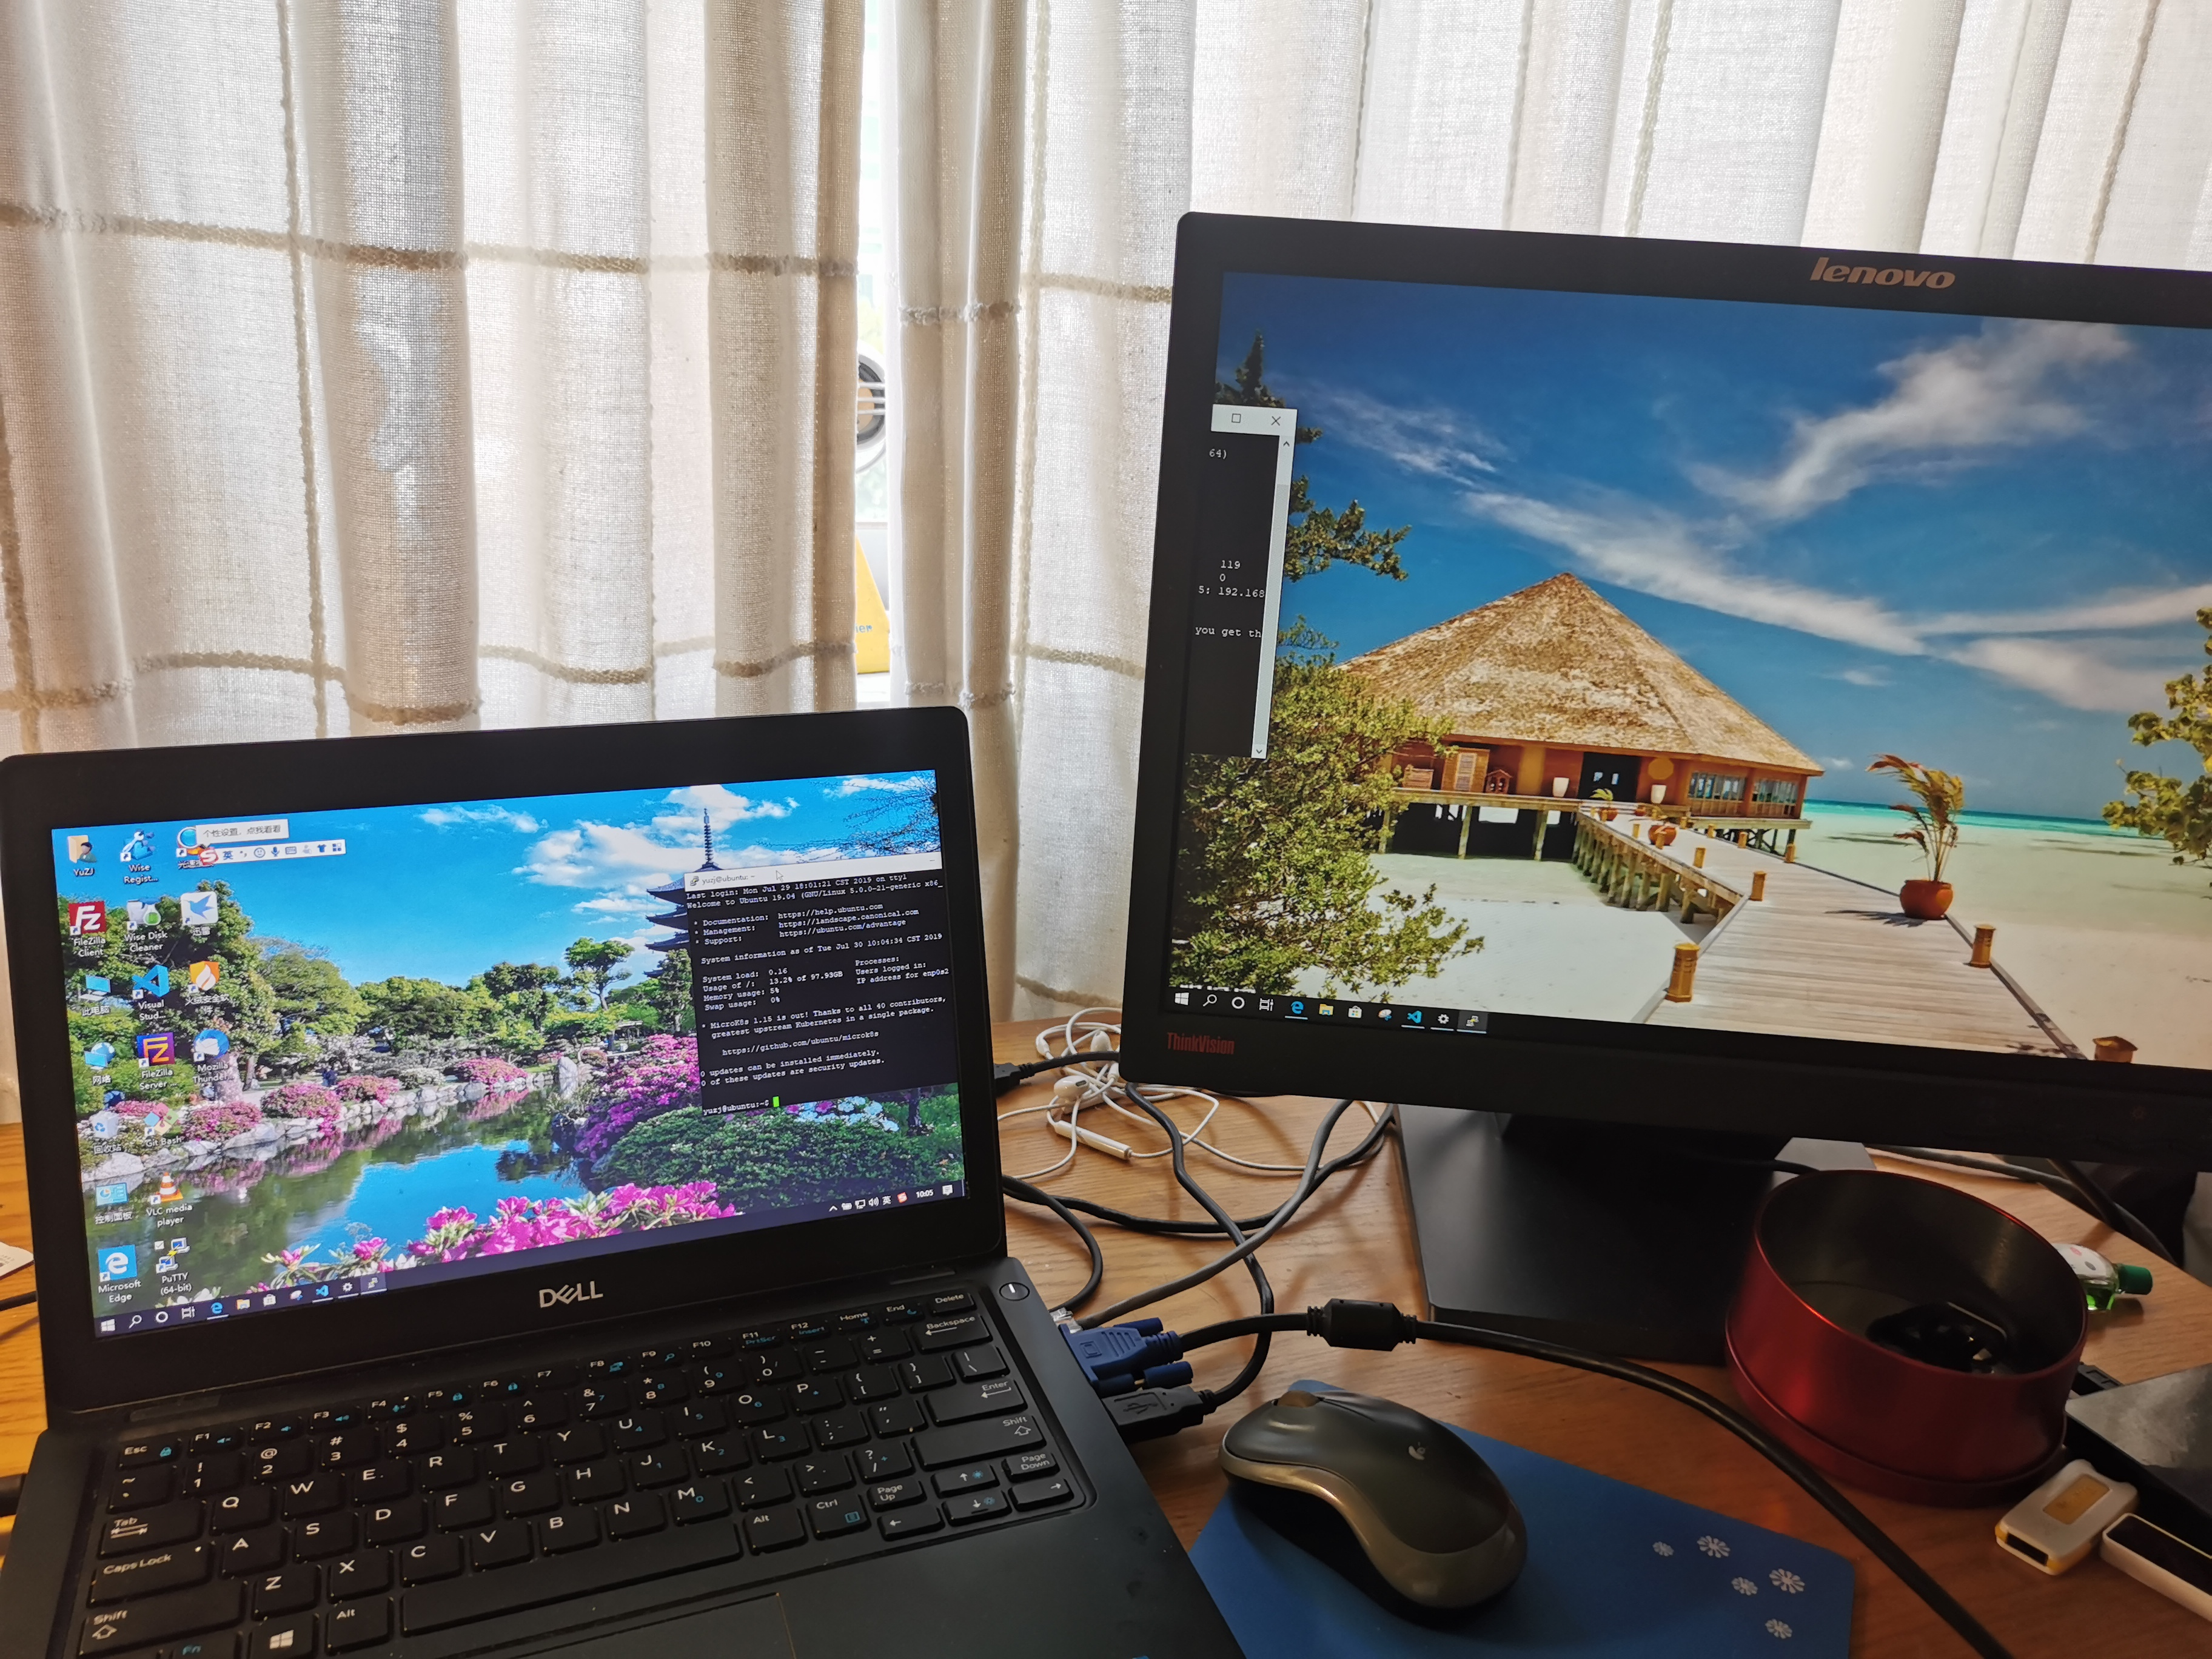
\includegraphics[scale=0.08]{pic/ScrExtend}
\end{center} 
\subsection{桌面(Desktop)、任务栏与开始菜单}
\begin{center}
	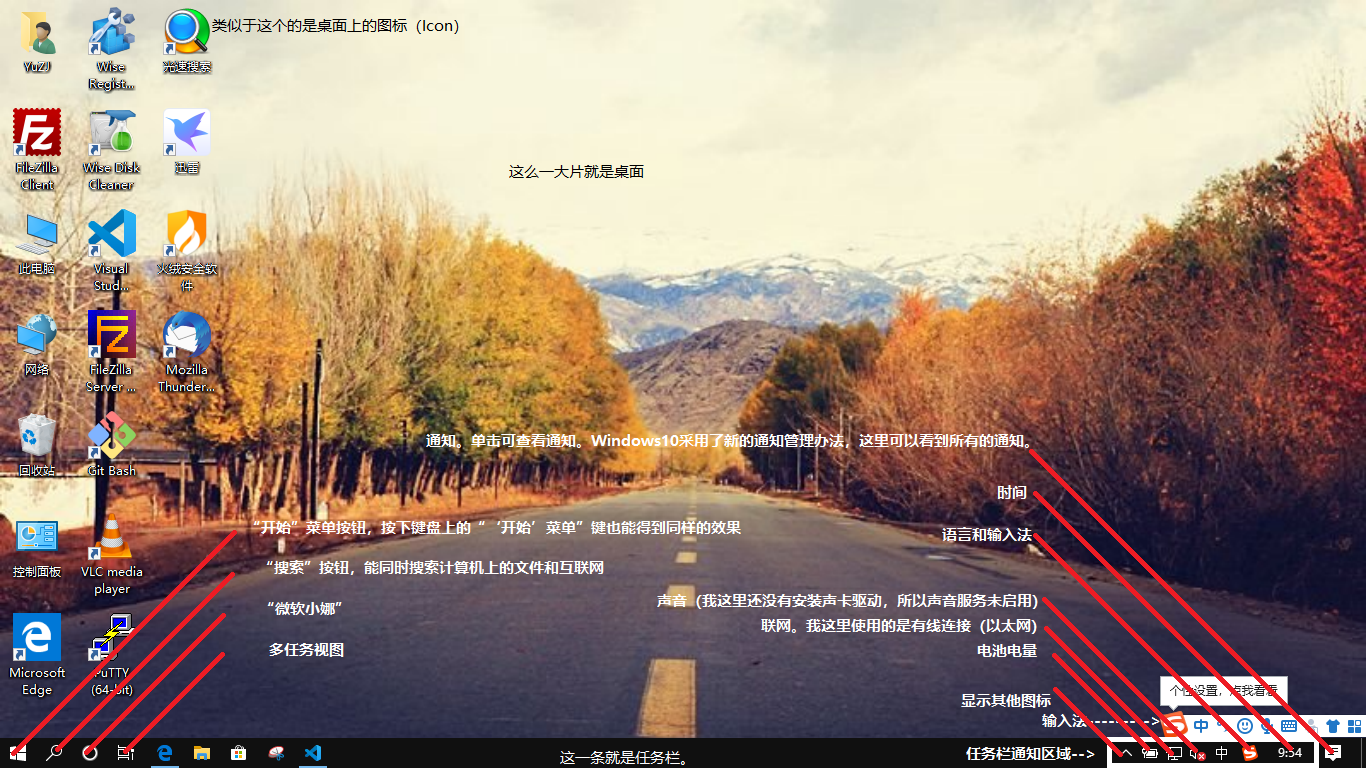
\includegraphics[scale=0.4,angle=90]{pic/screenIntro}
\end{center} \par
上图大致地概括了桌面、任务栏与开始菜单的组成部分。你可以自定义任务栏上显示什么图标。方法:在任务栏上右击-“任务栏设置”-“选择哪些图标显示在任务栏上”。
\subsection{窗口(Window/Form)}
\label{sec:Frm}
我们把屏幕上的一个一个独立的矩形区域称作“窗口”。比如说,这就是一个窗口:
\begin{center}
	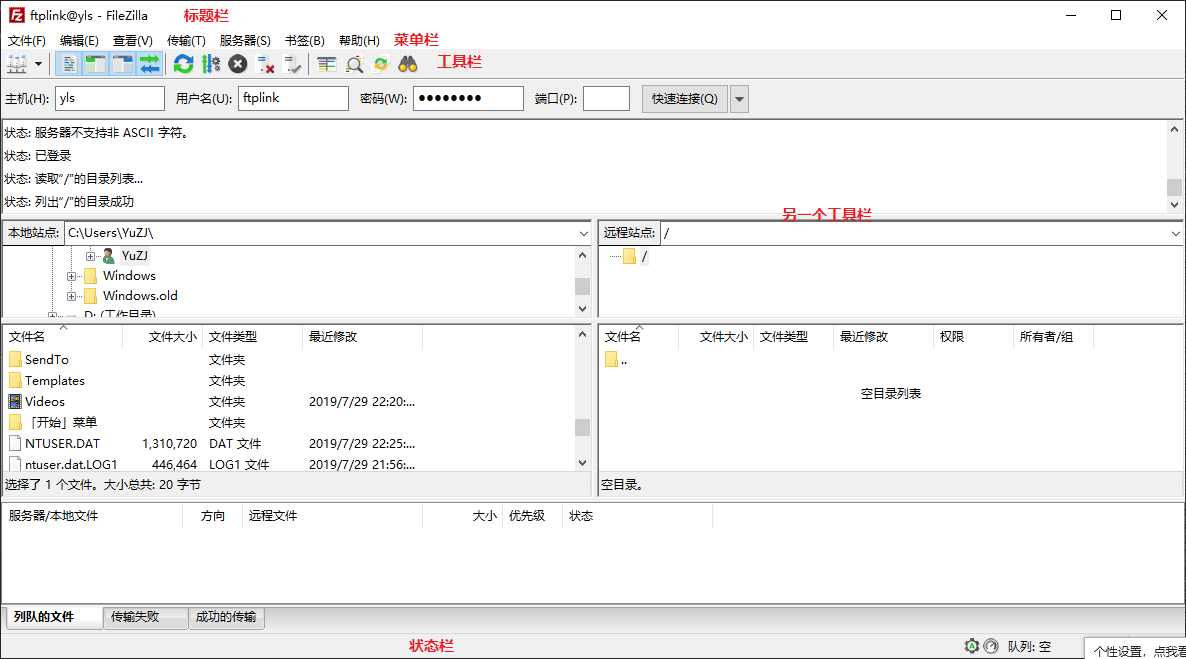
\includegraphics[scale=0.3]{pic/kj1}
\end{center} \par
一个窗口上面又有许多独立的组成要素,我们把它称为“控件”。常见的控件如下:
\begin{center}
	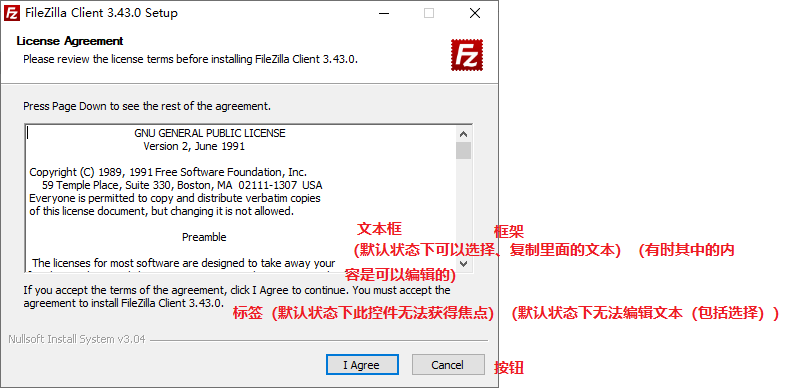
\includegraphics[scale=0.4]{pic/kj2}\\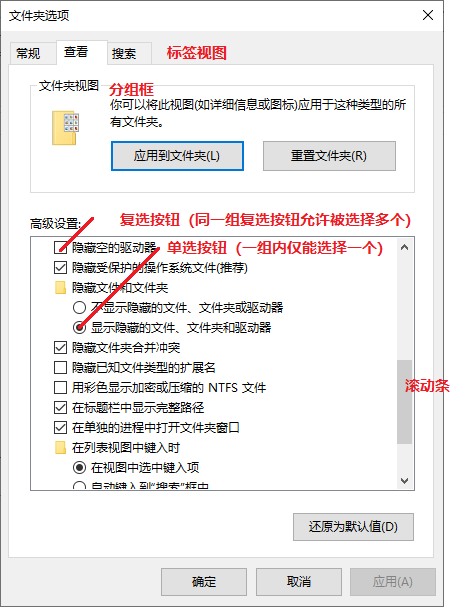
\includegraphics[scale=0.5]{pic/kj3}
\end{center} \par
现在请回到“键盘”学习如何使用快捷键。注意,有时它们又被称为“窗体”或“窗格”。
\subsection{文件(File)、目录(Directory)、路径(Path)与文件夹(Folder)}
简单地说,你在“文件资源管理器”上看到的不是文件夹的就是文件。文件夹在“详细信息”窗口与“属性”菜单中被清楚地标明“文件夹”。文件夹可以包含文件。现阶段你可以理解“文件夹”就是“目录”,虽然两者实质上是有区别的(目录是列表,文件夹是对象)。“路径”就是文件夹或者文件的“位置”,是一个字符串,如“C:\textbackslash Users\textbackslash SGComputers\textbackslash AppData\textbackslash Roaming\textbackslash Adobe\textbackslash Flash Player\textbackslash NativeCache”。Windows上使用“计算机-磁盘-文件(夹)”来管理文件。它们的路径包含设备卷标,如“D:\textbackslash”。关于绝对路径与相对路径你可以参考\pageref{sec:path}页的\ref{sec:path}。
\subsection{系统的关键位置}
目前阶段,这些关键位置的文件希望你不要操作:
\begin{enumerate}
	\item C:\textbackslash Windows  Windows操作系统放置系统可执行文件的地方。
	\item C:\textbackslash Windows\textbackslash System32  也是Windows操作系统放置系统可执行文件的地方。
\end{enumerate}\par
这些位置也比较重要:
\begin{enumerate}
	\item C:\textbackslash Program Files Windows操作系统应用程序的安装目录。这里安装的程序默认是可以被所有用户使用的。
	\item C:\textbackslash Program Files (x86) 如果你有这个目录,那么你的操作系统就是64位的。这里放置了32位应用程序的安装目录,而上一条中的目录是给64位程序使用的。如果没有,那么你的操作系统就是32位的。上一条中的目录是给32位程序使用的。
	\item C:\textbackslash ProgramData  存放在以上两个目录中的应用程序存放数据文件的地方。这里经常会有卸载残留,需要手动清扫(警告!只是删除自己熟悉且完全确定的目录)。
	\item C:\textbackslash Windows.old  老版本Windows的目录,如果不要回退到以前的版本你可以删除它(不要在“文件资源管理器”中删除——使用“开始”菜单-“Windows管理工具”-“磁盘清理”,使用管理员权限运行清理,删除“以前的Windows安装”)。
\end{enumerate}
\subsection{可执行文件(Executables)}
\label{sec:exe}一般扩展名为*.EXE,*.dll(Windows运行库文件)或*.COM(MS DOS可执行文件)等。一般地,仅二进制文件可在Windows操作系统上运行。虽然*.BAT(批处理文件。你可以把多个命令写入一个批处理文件并让Windows按照预定次序,满足预定条件地一次执行所有命令),*.CMD(类似于批处理文件,支持更多的命令,仅在Windows2000以上可用),*.VBS(VB Script,一种类似于VB的脚本语言),*.VBE(加密的VBS),*.JS(Java Script),*.JSE(不用说了吧),*.WSF,*.WSH,*.MSC(微软控制台文件)等文件也可直接在Windows操作系统上运行,但他们需要解释器。\par
可执行文件是系统必须的(系统启动的关键进程也是靠可执行文件完成的——你的桌面其实也是一个可执行文件的进程),但也是危险的。因此请不要删除系统关键位置的可执行文件(当然我也不相信你删得掉——有个叫做System的用户会阻止你的如果出现了病毒,反病毒软件会帮你删除的)并{\color{red}千万别双击自己不明白的可执行文件!!!!!!}下一节将会教你修改“文件资源管理器”的相关设置以防范虚假扩展名欺骗。
\subsection{-快捷方式}
快捷方式指的是一个指向目标文件的链接。
\section{-文件资源管理器}
\label{Sec:FE}
\begin{center}
	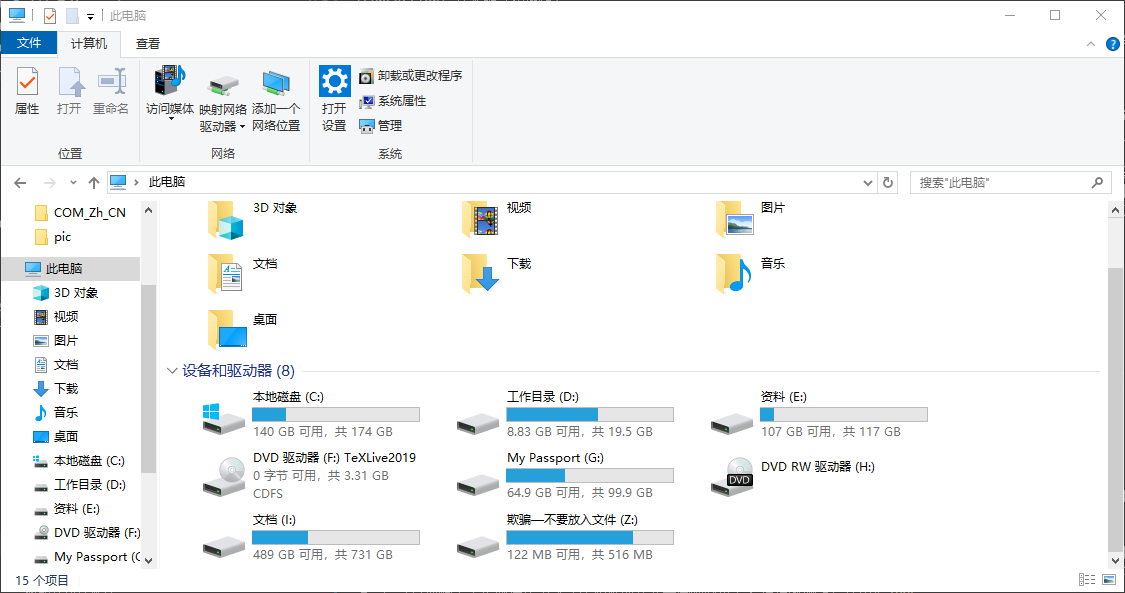
\includegraphics[scale=0.3]{pic/explorer}
\end{center} \par
“文件资源管理器”是什么?双击“此电脑”,你将得到一个文件资源管理器窗口。这就是“文件资源管理器”吗?\par
其实,事实不止于此。“文件资源管理器”位于“C:\textbackslash Windows\textbackslash explorer.exe”,是整个桌面系统的登录Shell(换句话说,“桌面”就是文件资源管理器的一个进程),一部分操作(如“控制面板”)也依赖于这个程序。因此如果你在任务管理器中结束了这个进程,你会发现桌面也消失了。\par
\subsection{反病毒和其它基本设置}
文件管理器是计算机安全的“兵家必争之地”,它的安全非常重要。因此,请注意“文件资源管理器”默认隐藏已知的扩展名,这就极易导致虚假扩展名欺骗。它的工作原理类似于这样:比如说现在这里有一个文件名为“1.bmp.exe”的文件。由于文件资源管理器认识“.exe”这个扩展名,文件资源管理器将显示为“1.bmp”。你知道“.bmp”是一个图像文件的扩展名,因此你双击希望打开它——就这样你中毒了。现在我们需要做的是强制文件资源管理器显示所有的扩展名。打开一个文件资源管理器窗口(如“此电脑”),选择“查看”标签-“选项”,取消勾选“隐藏已知文件类型的扩展名”并选择“显示隐藏的文件”(注意!不要取消勾选“隐藏受保护的操作系统文件”!对于一个初学者,我建议所有的系统文件应该被隐藏),单击“确认”即可。
\begin{center}
	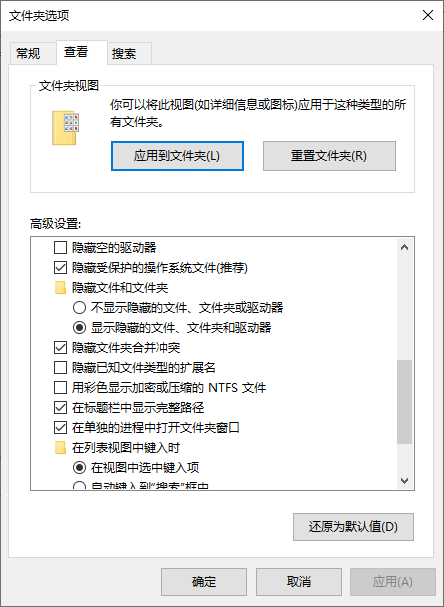
\includegraphics[scale=0.4]{pic/expset}
\end{center} \par
\subsection{-文件基本操作}
\paragraph{-资源管理器标签}
“标签”指的是资源管理器最上面的部分。我们主要讲3个标签:“文件”按钮、“主页”标签与“查看”标签。
\begin{center}
	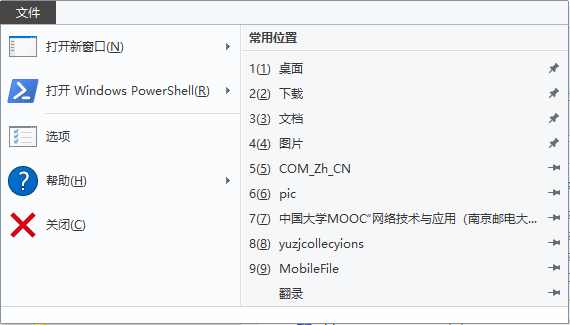
\includegraphics[scale=0.4]{pic/Exp4}
\end{center} \par
如图就是“文件”按钮。一般这里的常用项是“常用位置”显示的文件历史记录(右边一栏)、打开新窗口与打开Powershell。其中的“选项”按钮与“查看”标签的“选项”按钮相同。
\begin{center}
	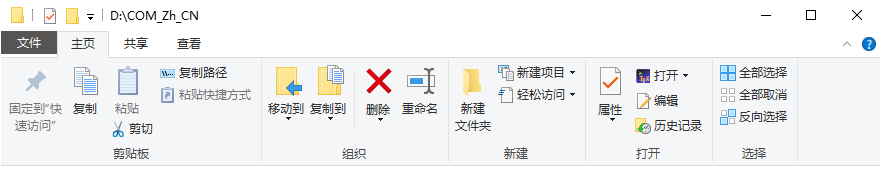
\includegraphics[scale=0.4]{pic/Exp9}
\end{center} \par
如图就是“主页”标签。你可以观察到标签上有多个“组”,我们一组一组来。\par
\begin{enumerate}
	\item “剪贴板”:“固定到‘快速访问’”对文件夹有效,它将把文件夹固定到右侧树状列表的“快速访问栏”(注意!不是“任务栏”)。“复制”与“剪切”就是将文件(夹)的{\color{red}路径}放入文件剪贴板中;“粘贴”为读取文件剪贴板上的路径来找到需要复制或剪切的文件,将它拷贝一份到当前目录再清空剪贴板(如果是剪切操作将删除源文件)。请注意“复制”或“剪切”文件后在“粘贴”前若删除源文件,“粘贴”将失效;对于一次“复制”或“剪切”操作,“粘贴”操作也不能进行2次。“复制路径”就是将当前文件的路径复制到系统剪贴板中,“粘贴快捷方式”是在当前文件夹创建被复制的文件(夹)的快捷方式。
	\item “组织”:我们一般只使用“删除”和“重命名”。
	\item “新建”:“新建”就是在当前文件夹中添加一个新的。这与右键菜单“新建”项是相同的。
	\item “打开”:你可以使用默认选项打开文件(夹)、查看文件(夹)属性或更改打开方式。另一种修改方法是右键单击某个文件,你将会发现“打开方式”菜单。若菜单标题为“打开方式(H)    >”那么这个文件已经有打开方式,你应在它的子菜单中选择打开方式。如果没有你需要的打开方式或标题为“打开方式(H)....”,那你就应该选择“选择其他应用”。一个对话框将会被显示(如下图)此时你需要使用鼠标滚轮向下滚动直至底部。如果没有发现你想要的应用,单击“更多应用”;还没有,单击“在这台电脑上查找其他应用”。此时你就需要知道你需要的应用的具体位置。一般应用程序位于“C:\textbackslash Program Files”“C:\textbackslash Program Files(x86)”“C:\textbackslash Users\textbackslash [用户名] \textbackslash AppData”的相应子目录或在安装时你自己指定的目录。{\color{red}为了避免这个问题,你需要在安装程序时记下安装位置。}如果出现了无法修改打开方式的问题,请尝试清理注册表(参见\pageref{sec:usab}页\ref{sec:usab})或杀毒。
	\item “选择”:更改文件的“选中”状态。你可以按住Shift键选择首末两项来选择它们与它们之间的所有项或者按住Ctrl键选择多项。
\end{enumerate}\par
\begin{center}
	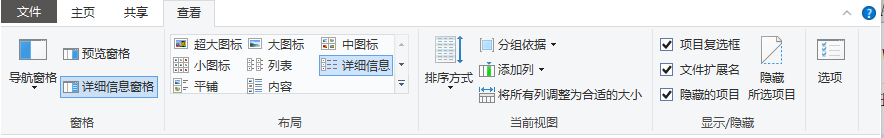
\includegraphics[scale=0.4]{pic/Exp2}
\end{center} \par
如图就是“查看”标签。
\paragraph{-右键菜单}

\begin{center}
	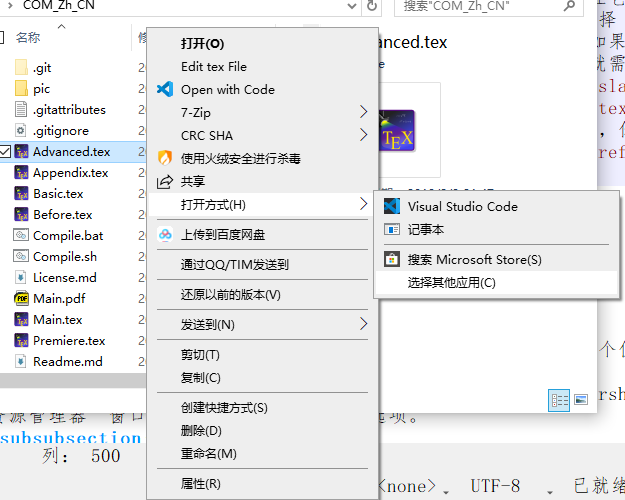
\includegraphics[scale=0.5]{pic/htopen1}  	\\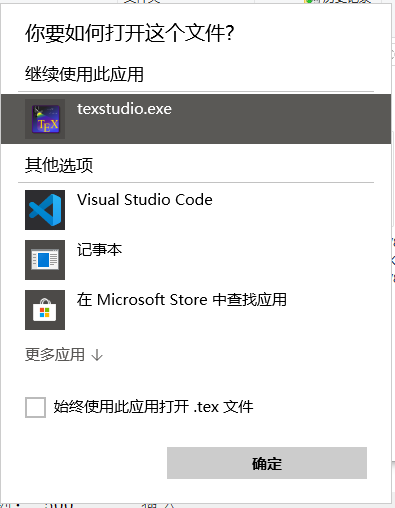
\includegraphics[scale=0.5]{pic/htopen2}
\end{center} 
\subsection{回收站以及Windows系统删除文件机制}
首先,请注意这里的“删除文件”仅限于使用文件资源管理器,不包括命令方法(如“DEL”或“rm”命令)。\par
当我们配置好一块硬盘时,所有能被Windows支持的分区上都自动创建了一个称为“回收站”的虚拟的区域。此时如果我们对大小小于该回收站的文件(夹)进行“删除”操作,这个文件就会被移动到回收站。此时如果我们在回收站里面执行“删除”操作或者清空回收站,这个文件就被永远删除了。但真的是这样的吗?\par
众所周知,文件是靠在磁盘上写入二进制数据保存的。此时如果我们删除一个文件,这个文件在磁盘上的位置其实是不变的——只是这个文件的属性被更改为“已删除”而已。此时如果回收站需要恢复文件只需要去掉“已删除”的标记即可。那么“清空回收站”是如何操作的呢?很简单,这个文件占据的区域被改为“可写”不再占据磁盘位置,其它文件可以被覆写在它的上面。\par
所以我们说即使你清空回收站,这个文件还是可以恢复的。此时如果你需要彻底删除它最好的办法是多覆写。你可以使用专业磁盘擦除工具来擦除磁盘。
\section{命令提示符}
\begin{center}
	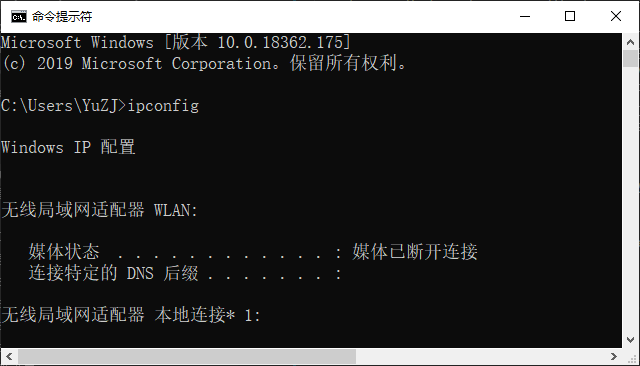
\includegraphics[scale=0.4]{pic/cmd}
\end{center} \par
如图,这就是命令提示符其实与GNU/Linux类似,这个窗口实质上是一个伪终端。你可以使用“开始”-“Windows系统”-“命令提示符”来访问它。\par
我们有时也会用到Powershell。你可以使用“开始”-“Windows Powershell”来访问它。大部分“文件资源管理器”窗口的“文件”菜单都有这个选项。
\section{网络连接}
首先请你咨询一下本地电教员以及班主任以确定教室内是否配备互联网以及(如果有)防火墙、时间控制与流量控制。\par
如果你的班主任思想比较落后,你可以自己联网。你需要一张无线网卡、无线网卡的驱动程序(这可以在网卡生产商处下载)和移动热点(或者,你也可以私拉网线——如果你们学校准许的话)。移动热点可以是手机(如果你们学校准许的话)或者无线上网宝(你需要一张流量充足的4G卡。如果你能忍受那个速度的话,3G也可以)。具体请参照手机“设置”以及上网宝说明书。\par
现在假设你已经配置好无线热点和网卡,现在寻找任务栏上的网络连接,你将发现你的无线网络并连接它。否则,检查驱动程序。下图的网络同时连接有有线以太网和Wifi。
\begin{center}
	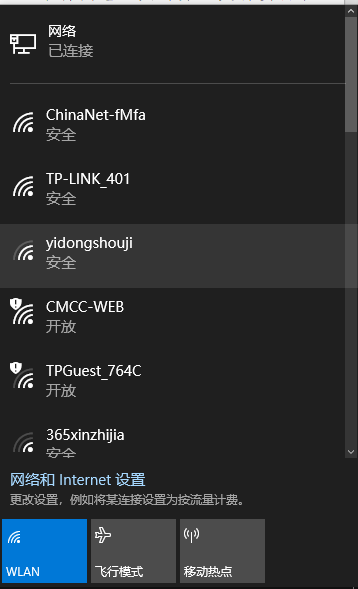
\includegraphics[scale=0.4]{pic/wifi}
\end{center} 
\section{-控制面板与设置}
\section{-任务管理器与资源监视器}
\section{-管理磁盘}
\subsection{-分区}
\subsection{-磁盘碎片}
\section{激活操作系统和自动更新}
如果你的计算机自带激活(比如说DELL的机器),Windows副本将在安装完后自动被激活。否则,你就需要输入序列号。使用未授权的KMS或其它破解行为违法并极易“引狼入室”,在这里不描述。如果你的工作组有Windows激活服务器(合法的KMS服务器)或者你的组织已经替你购买了正版操作系统(比如说浙江大学国际校区),请请教电教员。\par
你需要设置自动更新。如果你的工作组有Windows更新服务器,请请教电教员。否则,如果连接外网,Windows将自动更新。Windows更新将会提供最新的安全补丁,安装它们有利于提升电脑安全性。以前横扫世界的“冲击波”病毒只攻击没有安装特定型号补丁的旧型号Windows操作系统。不建议从第三方(如火绒“漏洞修复”)安装补丁。
\chapter{反病毒软件}
安装反病毒(antivirus)软件是重要的。它能够有效防止计算机病毒。
\section{如何选择?}
首先,最重要的当然是性能,其次是费用(免费优先),再次是易用性。我们可以从反病毒软件评测机构如AVtest \url{https://www.av-test.org/en/}(最后连接于2019年06月20日18:18:09)中得到他们的数据(以下数据来源:\url{https://www.av-test.org/en/antivirus/home-windows/}(最后连接于2019年06月20日18:20:04)):
\begin{center}
	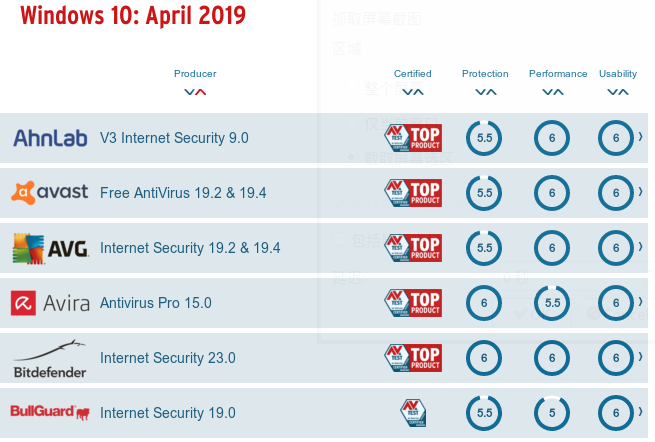
\includegraphics[scale=0.4]{pic/avtest1}\\
	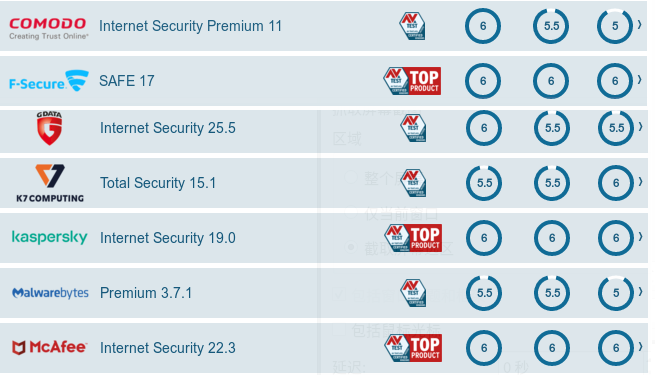
\includegraphics[scale=0.4]{pic/avtest2}\\
	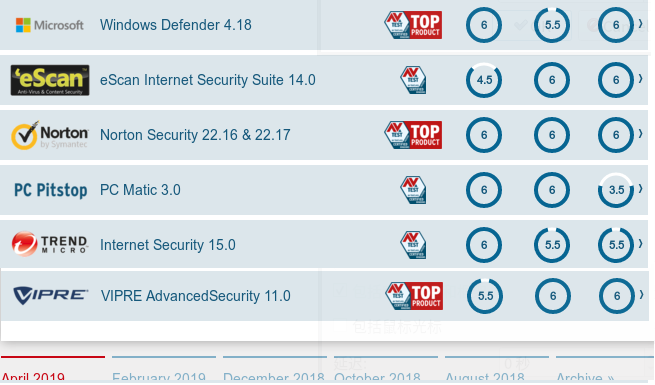
\includegraphics[scale=0.4]{pic/avtest3}
\end{center} \par
或者AV-Comparatives(地址:\url{https://www.av-comparatives.org/latest-tests/}(最后连接于2019年06月20日18:22:28))中的病毒移除能力测评数据(来源:\url{https://www.av-comparatives.org/tests/malware-removal-test-2018/#result-details}(似乎有些落后,不过没关系)(最后连接于2019年06月20日18:32:20)):
\begin{center}
	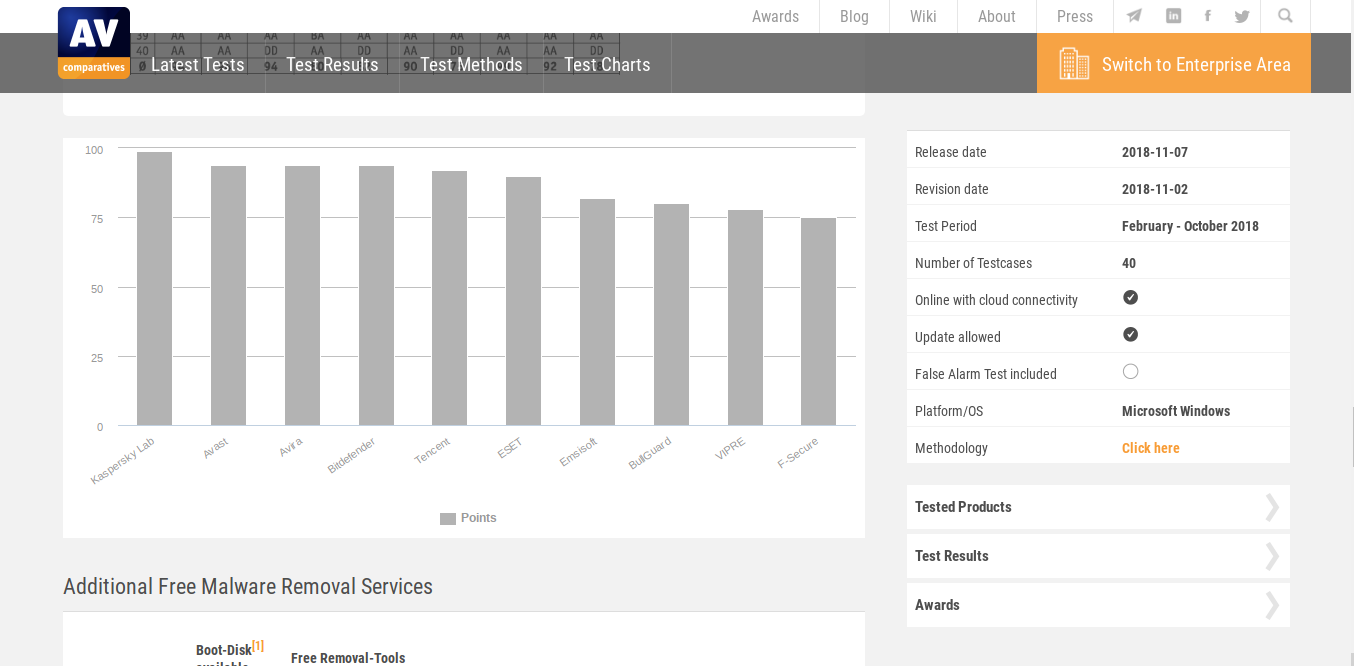
\includegraphics[scale=0.17]{pic/avc}
\end{center} \par
注意,你应该关注“家用Windows10产品”,而不是“企业”。\par
现在也许你会问一个问题:360在哪里呀?我不得不遗憾地告诉你:360由于送检产品与实际用户可以获得的产品存在不符,已经在AV-Test、AV-C机构黑名单上了。AV-Test最后一次测试于2017年10月,参见\url{https://www.av-test.org/en/antivirus/home-windows/manufacturer/qihoo-360/}(最后连接于2019年06月20日18:33:02)。AV-C最后一次测试位于2016年,参见\url{https://www.av-comparatives.org/vendors/qihoo/}(最后连接于2019年06月20日18:33:12)。
\section{教学用免费反病毒软件排行榜}
综合以上评测机构的数据加以自身使用经验,推荐以下反病毒软件:\footnote{说明中的wine指的是原生wine,不是deepin-wine。}\par
1.卡巴斯基免费版\par
地址:\url{https://www.kaspersky.com.cn/downloads/thank-you/free-antivirus-download}(最后连接于2019年06月20日18:33:26)。\par
优点:反病毒能力强劲,自我保护功能极强,病毒库更新快,支持任务计划及静默操作,中国用户支持好。\par
缺点:免费版功能有限,且对于配置较低的的计算机来说,“文件反病毒”功能消耗资源过大(意思就是说,有时会卡住)。扫描时占用系统资源极大。\par
注意:关于论坛上“卡巴斯基无法激活”或“无免费版”:请查看发帖日期和对应软件版本。这是一个较新的东西。
\begin{center}
	
\includegraphics[scale=0.3]{pic/kfa}
\end{center} \par
2.avast防病毒软件\par
地址:\url{https://www.avast.com/zh-cn/download-thank-you.php?product=FAV-ONLINE\&locale=zh-cn},最后连接于2019年06月20日18:34:13。\par
优点:反病毒能力强劲,支持任务计划及静默操作,中国用户支持好。\par
缺点:外媒声称存在推广安装,不断要求你购买付费版有点烦。
\begin{center}
	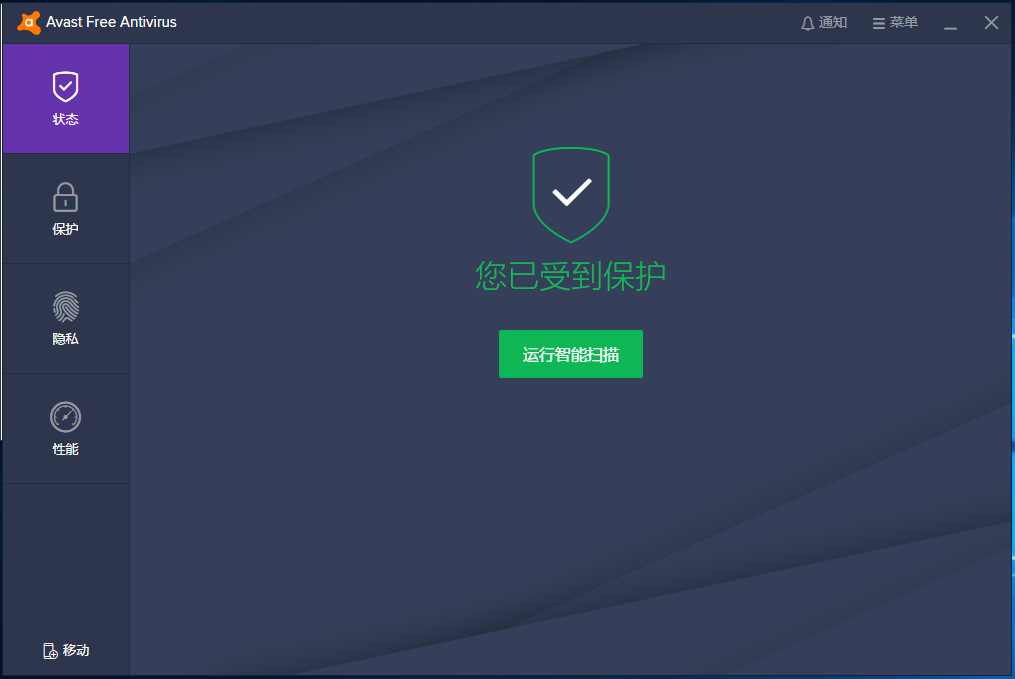
\includegraphics[scale=0.25]{pic/avast}
\end{center} \par
3.Avira Free Antivirus 2019\par
地址:\url{https://www.avira.com/zh-cn/free-antivirus-windows}(最后连接于2019年06月20日18:34:24)。\par
优点:反病毒能力强劲,自我保护功能强,病毒库更新快,支持任务计划及静默操作,中国用户支持较好,设置较为简易(主要是帮助详细)。\par
缺点:界面不美观,扫描时占用系统资源较大,不断要求你购买付费版有点烦。\par
下面显示的是Avira控制台、Avira反病毒软件及扫描画面(那个。看过《星球大战》的同学应该有所反应(Luke Skywalker与Luke Filewalker))。
\begin{center}
	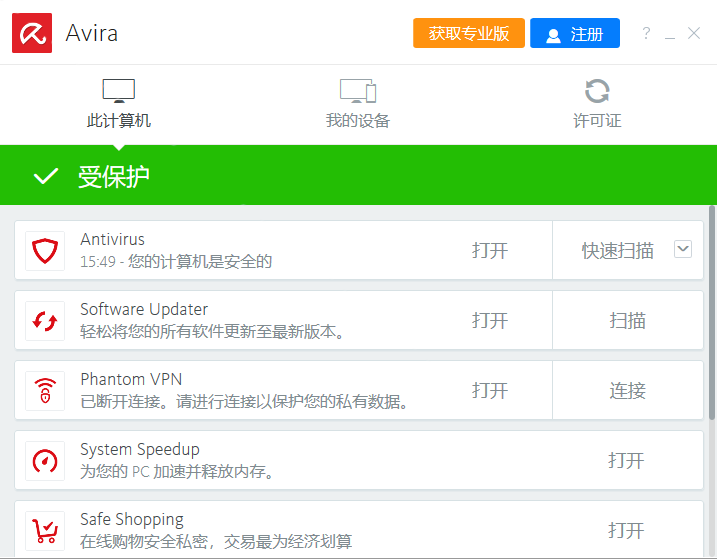
\includegraphics[scale=0.5]{pic/avi1}\\
	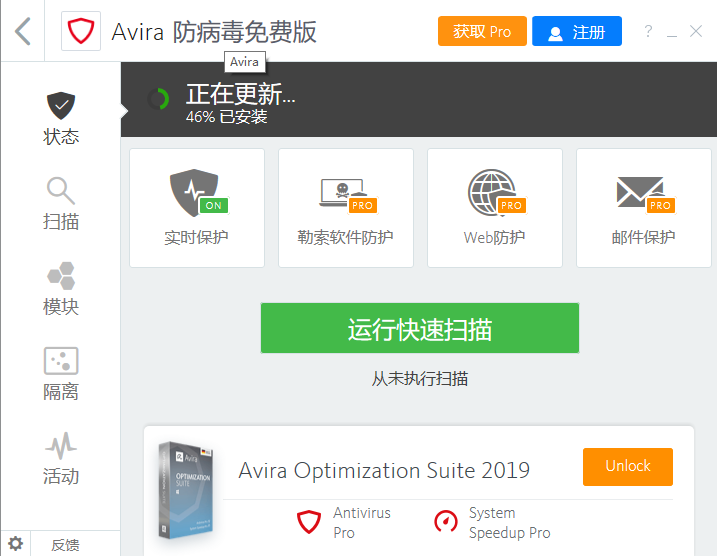
\includegraphics[scale=0.5]{pic/avi2}\\
	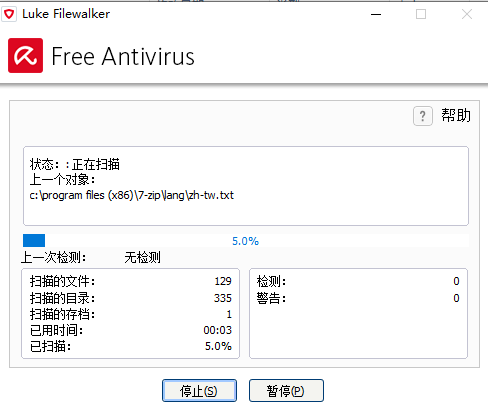
\includegraphics[scale=0.5]{pic/avi3}
\end{center} \par
4.火绒安全软件5.0
地址:\url{https://www.huorong.cn/}(最后连接于2019年7月30日09:23:43)。\par
优点:具有极强的HIPS(主机入侵防御系统,一种可有效防止计算机被入侵的机制)功能,有效拦截各类弹窗(如果开机启动(有时迟到)就基本没问题。如果无法拦截弹窗请先检查启动项)中国用户支持极好(废话,本来就是国产的嘛),占用体积小,可以被Wine来为GNU/Linux反病毒。\par
缺点:不参加世界安全软件测试,查杀能力略逊,反病毒“资历”尚浅。
\begin{center}
	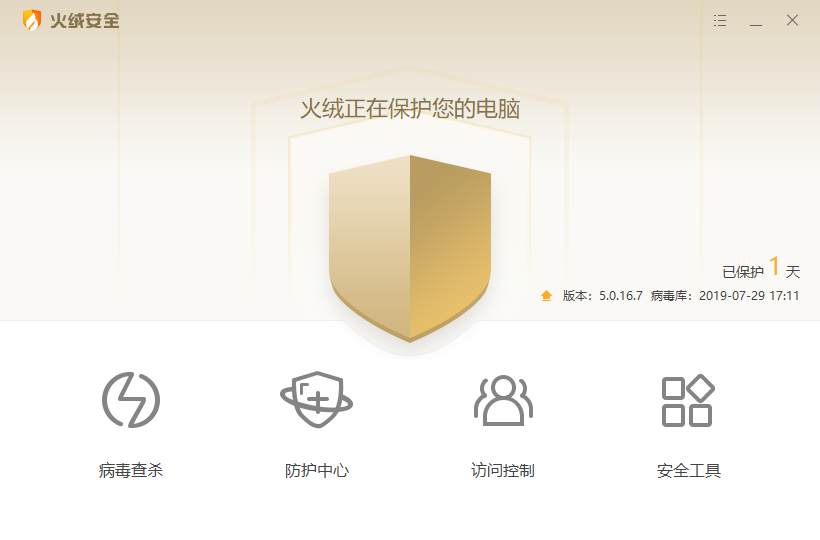
\includegraphics[scale=0.4]{pic/huorong}
\end{center} \par
5.腾讯电脑管家V13\par
地址:\url{https://guanjia.qq.com/}(最后连接于2019年06月20日18:34:53)。\par
优点:反病毒能力强劲,病毒库更新快,中国用户支持极好(废话,本来就是国产的嘛),可以被Wine来为GNU/Linux反病毒。\par
缺点:小工具过多(这个似乎是国产“杀毒软件”的通病),误报较为严重(这个似乎是反病毒软件通病)。
\begin{center}
	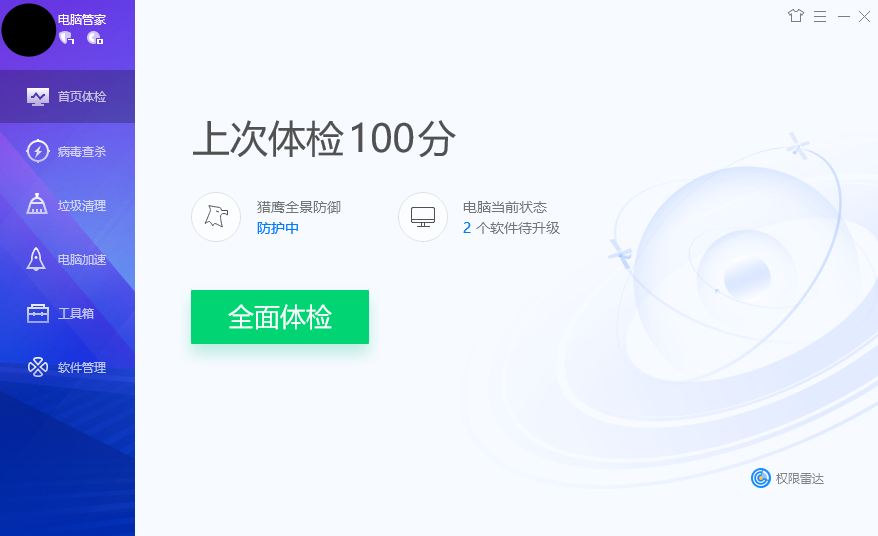
\includegraphics[scale=0.3]{pic/tsav}
\end{center} \par
6.360安全卫士12\par
地址:\url{https://www.360.cn/}(最后连接于2019年06月20日18:35:04)。\par
优点:中国用户支持极好(废话,本来就是国产的嘛),可以被Wine(易崩溃)来为GNU/Linux反病毒。多引擎联合查杀(安装有国外强大引擎),基于人工智能技术(360安全大脑)。\par
缺点:误报率较高,比如说我使用VB6.0编的小程序几乎都被报为病毒;如不经系统地设置会出现弹窗(有点烦;这似乎是国产软件的通病),安装体积较大。
\footnote{争议:360宣布退出AV-C事件。360官方宣布内容如下:传统杀毒评测标准落后云时代,我们正式退出AV-C 。日前国外杀毒评测机构AV-C联合AV-TEST、VB100宣称,360杀毒评测版本的引擎设置与国内普通用户版本不同,取消360在2015年评测奖项。对此我们认为,AV-C的传统杀毒测试方法已远远落后于云安全时代,双方无法就评测标准达成一致,360决定退出AV-C评测,并特此声明: 一、此次事件分歧是传统杀毒与云安全的评测标准之争。AV-C等机构成立于上世纪90年代,其评测标准也是基于传统杀毒技术而制定的。在AV-C看来,杀毒软件就应该是“特征码引擎+病毒库”,放在全世界任何一个角落都要测试出相同的结果,根本不认同云安全软件根据不同国家、不同地区配置更适应当地用户需求的引擎和云查杀防护策略; 二、360免费安全国际化触动传统杀毒行业利益。360杀毒以免费云安全模式在中国颠覆了传统杀毒市场。为开拓国际市场,360杀毒参加AV-C等国外评测,并多次获得全球最佳评级,测试版本的引擎设置一直公开体现在评测报告中,没有任何作弊行为。然而就在360免费安全国际化进程提速,并披露了国外用户数超过一亿的消息之后,国外的传统杀毒行业感受到了巨大挑战,AV-C也突然转变态度发出质疑,此举令我们无法接受; 三、AV-C传统评测标准远离用户真实需求。以国内某著名艺人网银被盗100万元的真实案件为例,不法分子骗其经纪人卸载了360杀毒,再要求受害者从钓鱼网站下载使用Teamviewer(一款世界知名的远程控制软件),从而控制其电脑盗取巨额网银资金。如果按AV-C评测标准,Teamviewer是合法软件,不应该“查杀”。而360杀毒集成了多引擎,其中QVM人工智能引擎对未知威胁的防护能力远远优于传统杀毒引擎,360云安全会根据文件下载途径、软件行为等信息综合判断并查杀被恶意利用的Teamviewer,这是传统评测所无法体现的、真正的安全保护;四、由于无法就评测标准和AV-C达成一致,360决定退出该项评测。事实上,赛门铁克、Comodo之前已退出AV-C,美国新兴的终端安全公司Bit9根本就没有参加这类评测。凭借全球领先的云安全技术和优秀的用户体验,360免费安全产品有信心在国际市场复制中国奇迹。 我们相信,最终的裁判是用户。 \par 不同观点:1.引用“科技行者”网站【360与AV-C之争背后 云安全时代评测标准需要革命】:\url{http://www.cnetnews.com.cn/2015/0504/3051837.shtml}(最后连接2019年6月19日11:27:53)。 (由于与360声明大致精神相符,以下内容已经被概括)AV-C标准落后,无法适用于云安全时代;360多杀毒引擎是为了更好实现地域化;中国杀毒产品的国际化正在受到落后的国际评测机制的制约;(以下为直接引用原文)“走出去是中国企业在国内做大做强之后的必然选择,360在确立自己的国际化战略之后,选择参加AV-C等国际评测,通过国际评测的成绩来增加产品在国际市场的影响力,在AV-C的评测标准无法准确衡量产品真正水平的情况下,不得不针对评测标准对产品进行妥协性设置,在不自觉中被AV-C这样的评测机构绑架,这也是360国际化付出的代价。国家互联网应急中心处长周勇林表示,中国市场与欧美杀软企业主导的外部市场已经形成了迥异的生态系统,中国杀软的商业模式是外国所不能适应的,但却被证明是有效的,很有竞争力;更重要的是,从企业综合实力看,中国企业做安全业务具备了动摇欧美老牌企业的体力甚至技术实力,因此,站在对方的立场上看,具备一定实力且熟练掌握新商业模式的中国杀软是很可怕的怪物,中国的杀软企业被“高度重视”是必然的,是可以理解的。希望360与AV-C的冲突事件,能够给中国企业国际化积累经验教训,目前国内杀毒软件厂商依然对国际评测趋之若鹜,但忽略了AV-C等国外评测机构与国外杀毒厂商是利益共同体这一事实,中国安全厂商想要进一步进入国际市场,势必与国际安全厂商成为竞争者,打压中国安全厂商是AV-C等机构的必然选择。互联网行业专家方兴东认为,中国安全企业的快速崛起和即将走出去的势头,必将严重威胁西方传统的安全企业,在话语权和主导权受制于人的情况下,中国要实现网络强国,强大的网络安全产业是重要基石,在产品、规则和评测等方面掌握话语权和主导权,也是必由之路。这需要我们尽快建立并扶植中国自主的云安全时代安全软件评测机构,建立安全软件的评测标准,掌握国际安全市场话语权。”。 \par  2.引用“太平洋汽车网”网站【退出AV-C 360愚弄了谁?】:\url{https://www.pcauto.com.cn/drivers/654/6545901.html}(最后连接2019年6月19日11:28:02)。(以下内容皆直接引用原文)奇虎360送检的产品与用户实际使用的产品并不相同;最终360承认了其产品在送测时被提前进行了修改;360的这份声明无疑是对广大360用户赤裸裸的愚弄;“AV-C成立于上世纪90年代,几乎与互联网同步发展,在杀毒检测领域有着丰富的经验,并已成为全球最权威的杀毒软件测评机构。AV-C测试方法是冻结杀毒引擎与病毒数据库三个月,并用最近三个月出现的最新病毒作为测试样本以检验软件杀毒能力,这种方法适用任意国家和地区,因为通过互联网传播的病毒并没有地域限制,而且该方法保证了对杀毒软件查杀最新病毒能力测试的准确性。360为了掩盖自身的问题强制将该问题转化为传统杀毒与云安全的标准之争是混淆视听。二、AV-C是非营利性公益组织,也是公认的国际性独立性测试机构,说360因为动了传统杀毒利益而挨刀显然站不住脚,因为AV-C并不代表着谁。而且,360以一家之言将非云查杀分为传统杀毒不过是为了抬高身份,事实上瑞金、卡巴斯基、金山、腾讯等都推出了云安全服务,AV-C也并没有收回他们的测评资质,360危机之时也不忘宣传自己也算罕见。三、Teamviewer不过是一个远程控制软件,只有双方同意的情况下方可使用,在各大软件下载网站都可轻易下载,因为使用Teamviewer而被盗显然不是软件本身的问题。事实上并没有哪家杀毒软件把它定义为非法软件,除了360。四、世界排名靠前的杀毒软件都不会拒绝AV-C的测评资质,也并不是所有的杀毒软件都可以接受AV-C的检测(因为AV-C测试门槛很高),赛门铁克、Comodo杀毒软件的退出不过是因为在AV-C的测评排名中比较靠后而已,以此来作为抨击AV-C的依据有失公允。”;“如果说AV-C评测落后,360从一开始就不会将自己产品送检,而在360产品出现问题并曝光之后才发布这样一份声明,其动机就已让人产生怀疑”。}
\begin{center}
	
\includegraphics[scale=0.3]{pic/360}
\end{center} \par
\begin{enumerate}
	\item 大多数国外反病毒软件之间相互兼容不好,只能安装一款。
	\item 同时安装过多的反病毒软件会导致计算机资源占用过多。
	\item “卡巴斯基免费版”-“设置”(左下角的齿轮)-“扫描”,设置“连接外部设备时”为“全盘扫描”(机器配置过低除外)(如果在扫描时你需要弹出磁盘,请先停止扫描。),“检测到威胁时操作”选择“删除”。这里的“删除”指的是移动到隔离区,“清除”是从文件中移除被感染的部分。
\end{enumerate}
在安装完反病毒软件后,你还要注意以下几点:
\begin{enumerate}
	\item 禁用“自动播放”。修改控制面板\textbackslash 硬件和声音\textbackslash 自动播放,取消勾选“为所有媒体和设备使用自动播放”,在“可移动驱动器”中选择“不执行操作”。
	\item 不能禁用UAC——即使也许这样会清净不少。对于不具有rootkit功能的病毒,UAC是你的最后一道屏障。
	\item 任何反病毒软件都需要更新——因此请在网络畅通时确保它们被更新了。或者你也可以使用离线更新包。火绒安全直接覆盖安装即可,卡巴斯基、小红伞等都有离线更新程序。
	\item 伪装成文件夹的病毒曾经多次出现。它将原来的文件夹隐藏起来,再伪装成一个WindowsXP文件夹引诱你点击。如果你点击的话,它就会在每块硬盘驱动器创建备份(感染它)并感染U盘。
\end{enumerate}
\subsection{在线分析文件}
VirusTotal是一个在线病毒分析网站,它可以调用多种反病毒引擎对上传的可疑文件进行检测。网址:\url{https://www.virustotal.com/gui/home/upload}(最后连接于2019年8月6日14:16:41)。
\begin{center}
	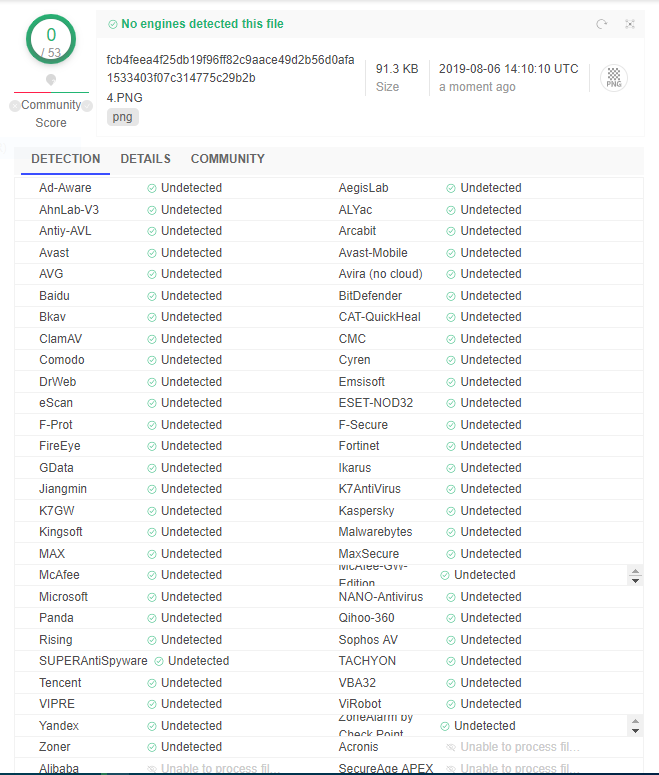
\includegraphics[scale=0.5]{pic/vt}
\end{center} \par
不过似乎有些反病毒引擎性能确实不太好(下图是微信2.6.8.65安装包和Ghost115)(欧洲著名反病毒软件Panda曾经将自己的病毒库当成病毒杀掉)。
\begin{center}
	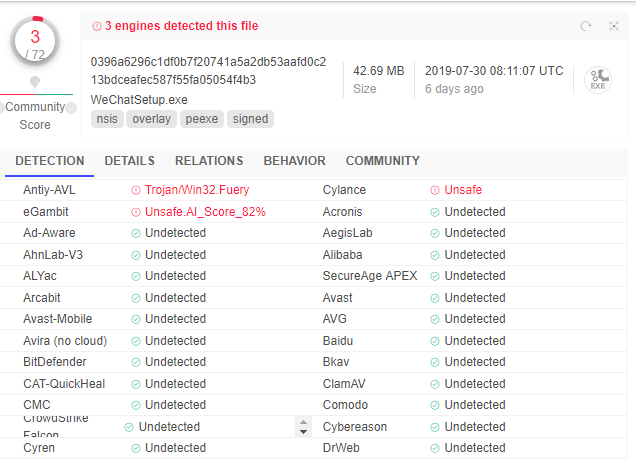
\includegraphics[scale=0.5]{pic/vt2}\\	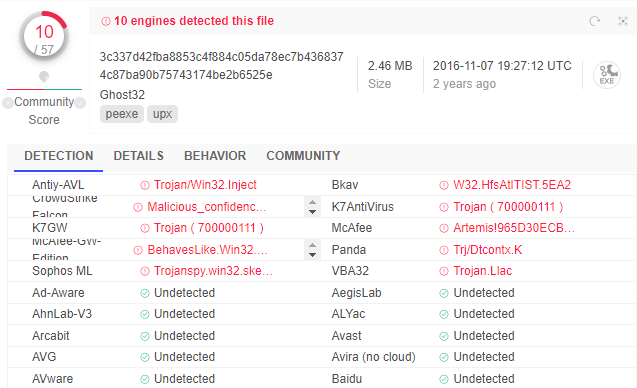
\includegraphics[scale=0.5]{pic/vt3}
\end{center} 
\chapter{压缩/解压缩}
对于压缩软件,大部分人都会想到WinRAR,我们使用7-Zip。\footnote{注意,我们暂时不讲国产压缩软件(如360压缩)。我认为掌握了难于操作的软件(7-Zip),操作容易的也自然能够被掌握。国产软件可能存在安全问题:【火绒安全-知名压缩软件"快压"传播病毒和多款流氓软件 劫持流量】\url{https://www.huorong.cn/info/1531309921141.html}(最后连接于2019年6月21日16:16:19)。当然也包括2345旗下产品——你安装任意一款就会被安装“全家桶”了。这里我们使用自由软件7Zip。}它虽然是自由软件,但性能极为优异。7Zip安装版可以在 \url{https://www.7-zip.org/download.html}(最后连接于2019年06月20日18:37:09) (英文官网),【7-zip官方中文主页】\url{https://sparanoid.com/lab/7z/}(最后连接于2019年06月20日18:37:38 )(中文官网)。你需要仔细观察。我建议下载EXE格式(当然某些大牛会下载源代码)的对应版本。\par
你将会发现7-Zip的安装界面十分简单。就像:
\begin{center}
	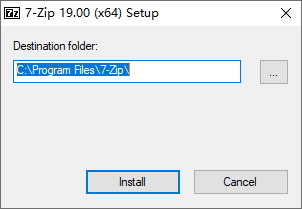
\includegraphics[scale=0.5]{pic/7zipinst}
\end{center} \par
在安装完成后,你需要手动设置文件关联(相当于设置一个或多个扩展名均使用此软件来打开。小资料:Windows操作系统在命令行中传送该文件的完整路径到预定的程序,这样程序就知道打开那一个文件了。Windows操作系统通过扩展名识别文件类型。这一点与GNU/Linux(靠文件内容识别文件类型)不同。一个文件可以没有扩展名,此时Windows会每次都让你选择打开方式。GNU/Linux会自动判断文件类型,自动选择)。你需要以管理员权限运行开始菜单的“7Zip File Manager”(它应位于安装目录的“7zfm.exe”)。选择“工具-设置”菜单,你将会发现如下界面:
\begin{center}
	\includegraphics[scale=0.5]{pic/7zopt.PNG}
\end{center} \par
在“系统”选项卡上单击二个标题为“+”的按键即可创建全部文件关联。对于Windows10,我建议取消“*.iso”文件关联而使用系统默认虚拟光驱。如果你安装了其它虚拟光驱也如此设置。单击“确定”保存。我们主要通过“文件资源管理器”右键菜单来处理压缩文件。对于压缩算法,我们曾进行过一个测试,结果如下:
\begin{center}
	\includegraphics[scale=0.4]{pic/ziprate.PNG}	
\end{center} \par
通过以上数据,我们认为最好的压缩算法是运用于7Zip的LZMA2(极限压缩)。\par
小资料:常见关于“设置”的英文表示。console——控制台 ,cmd——命令提示符,opition——选项,tool——工具,language——语言,preference——首选项,configure——配置。如果是英文界面就到这里去找吧。
\chapter{媒体播放器VLC}
由于版权争议\footnote{依照FFmpeg官方,国产播放器暴风影音、QQ影音被发现使用FFmpeg的解码器而并未按照FFmpeg许可证要求使用。以上厂商坚持认为他们的做法没有违背许可证。当然我也不得不说,GNU GPL也许是世界上最难理解的许可证之一。请参见【GNU许可证常见问题】\url{https://www.gnu.org/licenses/gpl-faq.html}(最后连接于2019年06月21日08:40:00)并咨询法律界专业人士(如专门从事知识产权及版权方面的律师)。}我们暂时不提国产播放器。我们使用自由的VLC。其界面如图所示。
\begin{center}
	\includegraphics[scale=0.4]{pic/vlc.png}	
\end{center} \par
同样是自由软件的还有MPV(界面简洁,操作难度较大,大部分需要键盘操作)与SMPlayer(对于配置较低的机器,它的性能不佳)。
\subsection{获取VLC}
你可以从以下网站获取VLC:官网【VLC:官方网站 - 全平台的自由多媒体解决方案! - VideoLAN】\url{https://www.videolan.org/}(最后连接于2019年06月25日08:25:14);Tuna源(64位)\url{https://mirrors.tuna.tsinghua.edu.cn/videolan-ftp/vlc/last/win64/}(最后连接于2019年06月25日08:26:01)。为简化安装,你应该下载exe格式安装包。
\subsection{使用VLC}
在默认界面(vlc有许多皮肤,甚至还有一个皮肤编辑器),VLC长得与其他播放器大同小异。但你可以自定义VLC的界面。方法:工具-自定义界面。请注意,最顶端的菜单条中的内容与在播放主界面中右键菜单调出的内容是相似的。\par
VLC也提供了许多高级功能。“视频”菜单项就“藏龙卧虎”。
\begin{enumerate}
	\item “缩放”:这个功能能改变视频尺寸(换句话来说,让视频播放窗口变小)
	\item “宽高比”:这个功能能够将视频“变形”以显示要求的宽高比
	\item “裁剪”:裁剪画面使符合要求的宽高比。这可在分辨率不符合要求时裁剪画面铺满屏幕。
\end{enumerate}
\chapter{-办公软件}
\section{MS Office}
名气最大,市场占有率最高,易用性最强的办公软件!Windows操作系统上目前主要版本由97(32位Windows10目前仍然可用的最早的版本)、2000、xp、2003(名气极大,新增InfoPath与OneNote)、2007(使用标签页菜单并删除frontpage)、2010(授权方式更改—你不能够使用一个不属于自己的序列号激活,最后一款支持WindowsXP的Office)、2013(开始位于Office365并且能够打开PDF和网页文件,新增Onedrive)、2016(开始产生电脑与手机、平板电脑联动的云办公时代)、2019(仅仅支持Windows10)以及免费的网页版(国内性能极差)。对于允许手机的学校,你也可以使用手机版本(包含Word、Excel、Outlook、OneNote、Onedrive与PowerPoint等,完全能满足教学需求)。\par
首先需要说明的是,正版的MS Office是需要收费的。具体收费标准参见Office官方网站\url{https://products.office.com/zh-cn/home}(最后连接于2019年7月28日16:31:18)。如果你的计算机自带激活(比如说部分DELL的机器),Office副本将在安装完后自动被激活。否则,你就需要输入序列号。如果你的工作组有Office激活服务器(合法的KMS服务器)或者你的组织已经替你购买了正版操作系统(比如说浙江大学国际校区),请请教电教员。
\section{自由/开源的办公软件}
对于不愿付款但希望使用正版软件的电教委员来说,一份自由/开源的办公软件是极好的。这类软件主要有Apache OpenOffice(开源软件,使用Apache许可证)与LibreOffice(自由软件,使用GNU GPL许可证)。由于二者操作极为相似,这里仅介绍LibreOffice。\par
你可以从它的官方网站\url{https://zh-cn.libreoffice.org/}(最后连接于2019年06月21日08:52:35)中下载最新版与离线中文帮助。从tuna源\url{https://mirrors.tuna.tsinghua.edu.cn/libreoffice/libreoffice/stable/6.2.4/win/x86_64/}(最后连接于2019年06月21日08:54:44)下载6.2.4版本64位软件包。具体解释如下:Stable是“稳定版”,“portable”版本可以被装进U盘随身携带。附上截图二张(已经启用标签页模式):
\begin{center}
	\includegraphics[scale=0.35]{pic/loffice_wr}
\end{center} \par
Tips:如果你需要LibreOffice产生类似于MS Office 2007以后的标签效果,你需要在“视图”-“用户界面”-“标签页模式”。\par
一部分扩展程序(如Writer2LaTaX)以及数据库软件(LibreOffice Base)需要Java运行库,你可以到\url{https://www.java.com/zh_CN/}(最后连接于2019年8月7日08:31:36)处下载Oracle JRE或者\url{http://jdk.java.net/12/}(最后连接于2019年8月7日08:31:26)处下载OpenJDK。LibreOffice支持两者而OpenOffice似乎仅支持前者。此时你需要到“选项”-“LibreOffice”-“高级”/“选项”-“OpenOffice”-“Java”设置Java运行库路径,一般是Java安装路径下的“bin”文件夹。
\section{-国产办公软件}
WPS毫无疑问是这里做得最好的。官方网站:\url{https://www.wps.cn/}(最后连接于2019年06月21日08:46:31)。还有另外一款永中Office,官方网站:\url{http://www.yozosoft.com/products/study.htm}(最后连接于2019年06月21日08:48:27)。均为免费下载,其中WPS与永中都有自己的文档格式(永中为“标文通”即UOF,知道的人可能不多)且兼容性都比较不错。
\section{-给我强大的生产力!}
\label{sec:OneDrive}通过网络协作,Office可以形成很强的生产力。
\subsection{文件共享}
这项功能一般可以通过云盘或者FTP来实现。注意,选择第三方云存储机构要考虑数据安全性,尽量选择有口碑的云服务提供商(如百度网盘)。微软OneDrive结合Office电脑端、手机端将会产生强大的生产力,你能够多端编辑。\par
局域网内可以使用FTP来共享文件。这里教你如何使用自由免费的FTP客户端Filezilla。官网:\url{https://filezilla-project.org/}(最后连接于2019年7月30日09:36:35)。在官网上你会发现“Download FileZilla Client”与“Download FileZilla Server”两个按钮,你应该选择前者(下载客户端)。否则你将会得到一个FTP服务器。请注意安装时勾选“Languages”以免出现英文界面。安装好启动后如图所示:\par
\begin{center}
	\includegraphics[scale=0.25]{pic/fz}
\end{center} \par
现在尝试连接网内的FTP服务器。向电教员询问FTP服务器的IP地址,你被分配的用户名、密码以及服务器端口号(这个一般是21)使用“快速连接”测试连接。如果你遇到了一个“保存密码?”的对话框,你应该选择“不保存密码”以增强安全性。一般情况下,在最上面的一个文本框内你将得到:
\begin{verbatim}
状态:	正在连接 192.168.0.101:21...
状态:	连接建立,等待欢迎消息...
状态:	不安全的服务器,不支持 FTP over TLS。
状态:	服务器不支持非 ASCII 字符。
状态:	已登录
状态:	读取目录列表...
状态:	列出“/”的目录成功
\end{verbatim}
若出现错误,请请教电教员。连接成功以后,你可以在“文件”-“站点管理器”里面添加这个站点。下次连接只需要在工具栏上的“站点管理器”下拉列表做出选择即可。如果你使用有线连接并且你的电教员水平极高(并且学校在这方面投入很大),你将得到大于10MB每秒的网速。Filezilla操作简便,你会发现左边是本地文件,右边是远程文件。大多数操作只需拖动即可完成。\par
Filezilla也可以被用于连接远程公共FTP服务器。
\subsection{带有版本控制的文件共享}
你是否需要一个能够记录你对特定文件(如一篇论文)所做出的所有更改的机制?那么一个版本控制软件能满足你的需求。在这里我们使用分布式版本控制软件Git。你可以从Git的官方网站\url{https://git-scm.com/}(最后连接于2019年8月10日11:14:32)下载Git,并在\url{https://git-scm.com/book/zh/v2}(最后连接于2019年8月10日11:15:27)下载官方中文帮助。
\subsection{-使用Office系列}
\chapter{文本编辑器}
文本编辑器就是能够编辑文本的计算机软件。它能够识别多种编码(如GB2312,UTF8等等)和断行格式,提供字数统计、语法高亮、替换等功能。文本编辑器是基础性的软件,任何计算机和编程者都需要文本编辑器。下面介绍几款常用且免费的文本编辑器,功能由上到下逐渐丰富。NotePad++作者由于多次发布反华信息,这里不再介绍其软件。
\section{Notepad}
\begin{center}
	\includegraphics[scale=0.4]{pic/winnotepad.PNG}	
\end{center} \par
Notepad又称“记事本”,是大多数Windows系统的必备组件。一般你可以在“开始”菜单-Windows附件中找到它。它安装于“C:\textbackslash WINDOWS\textbackslash system32\textbackslash notepad.exe”。\par
它能够执行一些诸如查找替换及字符统计这样简单的任务,是Windows系统上最简单的源代码编辑器之一。\par
值得注意的是保存文件时的编码方式:ANSI与UTF-8。一般用于Windows操作系统的文件(如,批处理文件)我们保存为ANSI,但大多数编辑器都支持UTF-8。\par
注意,打开部分文件时记事本无法正确地断行。这是由于Windows与GNU/Linux的断行符格式不同。Windows使用CR(回车)LF(换行),GNU/Linux仅LF,Macintosh仅CR。如果你经常使用那些从GNU/Linux上移植的软件(如GIMP,Git或GNU Emacs),你可以使用以下几款文本编辑器。
\section{Visual Studio Code}
开源软件--它使用微软公司软件许可证。
\begin{center}
	\includegraphics[scale=0.35]{pic/vscode.PNG}
\end{center} \par
“微软的另一款良心之作”。除了notepad++提供的功能外,还具有调试器以及完全自定义功能。其GNU/Linux版允许你调试Visual Studio程序。支持大量的文件格式以及扩展,扩展商店一级棒。下载:\url{https://code.visualstudio.com/}(最后连接于2019年8月9日20:35:04)。
\section{VIM}
自由软件。
\begin{center}
	\includegraphics[scale=0.4]{pic/vim.png}\par   \includegraphics[scale=0.4]{pic/gvim.png}
\end{center} \par
分别为终端模式与图形界面。
\subsection{下载安装}
其官方网站为\url{https://www.vim.org/}(最后连接于2019年06月20日18:38:36)(速度较慢);ustc开源镜像站镜像网址\url{http://mirrors.ustc.edu.cn/vim/}(最后连接于2019年06月20日18:38:46)。是一个十分强大的文本编辑器,公认类vi编辑器中最好的编辑器。注意:它的入门门槛较高。你需要记住大量命令。所有发行版的GNU/Linux默认安装vi,因此我建议学习高级部分的电教委员能学习一下这个编辑器。它的学习曲线较陡,但也值得迎难而上。\par
具体命令示例由于VIM较为复杂,这里不再赘述。(如果你发现自己无法退出,请单击“ESC”,键入“:qa!”并回车)但建议希望学习“高级”篇的电教委员学习一下。
\subsection{帮助及学习}
首先你应该学习“Vim Tutor”。进入方法:直接在终端或命令提示符中键入“vimtutor”并回车。这个教程有许多语言可供选择,默认匹配系统。\par
之后你可以学习“VIM USER MANUAL”这是vim最完全的用户手册。其中文安装版及pdf版可在\url{http://vimcdoc.sourceforge.net/}(最后连接于2019年06月20日18:39:21,速度较慢)中下载。直接下载链接:\url{https://sourceforge.net/projects/vimcdoc/files/win32-install-unicode/vimcdoc-2.1.0-setup-unicode.exe/download}(最后连接于2019年06月20日18:40:27,网速较慢)及\url{https://sourceforge.net/projects/vimcdoc/files/pdf-manual/reference-2.1.0.pdf/download}(最后连接于2019年06月20日18:41:03,网速较慢)。官方文档均可在\url{https://www.vim.org/docs.php}(最后连接于2019年06月20日18:42:01,网速较慢)中被找到。\par
我还推荐一个中国台湾的文档《大家來學VIM(一個歷久彌新的編輯器)》:\url{http://www.study-area.org/tips/vim/}(最后连接于2019年06月20日18:41:24)。
\chapter{文件搜索}
我们最擅长使用的“文件资源管理器”的搜索功能不是很强。现在我介绍一款文件搜索工具:光速搜索。截图:
\begin{center}
	\includegraphics[scale=0.5]{pic/finder}
\end{center} \par
它不负“光速搜索”美名,搜索真的快——只是在开始时需要建立搜索索引比较耗时。还可按扩展名进行搜索(请在左侧面板右击设置)。官网\url{http://finder.sdo.com}似乎暂时无法访问,提供安装包哈希校验。md5:896b3b93ce29b16c294884437ee11631 sha1:d7873a901d7cbb9fb1cf2bbd3a3c0a7e99f4f5f5 光速搜索1.0.1.280。
\chapter{性能工具}
\label{sec:usab}这就是国产“杀毒软件”(如腾讯电脑管家)的优势——它们的“清理优化”功能更适合中国消费者。现在介绍三款国外性能软件。使用十分简单,因此仅附上截图:
\begin{center}
	\includegraphics[scale=0.25]{pic/ccc}\\
	\includegraphics[scale=0.3]{pic/wdc}\\	\includegraphics[scale=0.3]{pic/wrc}
\end{center}
\section{CCleaner}
看起来好像是付费软件,但其实免费版功能已经够用了。官网:\url{http://www.ccleaner.com/ccleaner}(最后连接于2019年6月21日15:57:51)。直接下载:\url{https://www.ccleaner.com/ccleaner/download/standard}(最后连接于2019年6月21日15:58:27)(网速较慢)。\par
在下载完后运行安装程序,单击主界面的“自定义”,除了“添加到开始菜单”与“添加到桌面”保持勾选外,取消其余勾选。之后单击“安装”即可安装。\par
第一次启动时设置界面为简体中文(Chinese Simplified)(Opinion-Setting-Language),取消“智能清理”全部勾选,“自定义清理”中“Windows”除“高级”外全部勾选,“应用程序”全部勾选,单击“运行清理”即可清理。CCleaner还支持清理注册表、磁盘擦除以及软件更新提醒。
\section{Wise Disk Cleaner}
看起来好像是付费软件,但其实免费版功能已经够用了。下载:\url{https://www.wisecleaner.com/download.html}(最后连接于2019年6月21日16:09:32)。官网:\url{https://www.wisecleaner.com.cn/wise-disk-cleaner.html}(最后连接于2019年6月21日16:11:14)。除了一般清理功能以外还支持磁盘碎片整理。
\section{Wise Registry Cleaner}
看起来好像是付费软件,但其实免费版功能已经够用了。下载:\url{https://www.wisecleaner.com/download.html}(最后连接于2019年6月21日16:09:32)。官网:\url{https://www.wisecleaner.com.cn/wise-registry-cleaner.html}(最后连接于2019年6月21日16:10:42)。
\section{手动清理}
一般软件存在卸载后残留。此时你应该访问应用程序的安装目录\footnote{如果你忘了,我来提示你:“C:\textbackslash Program Files”“C:\textbackslash Program Files(x86)”“C:\textbackslash Users\textbackslash [用户名] \textbackslash AppData”}。你还应该关注“C:\textbackslash Program Data”以及各磁盘的根目录(比如说,腾讯视频与爱奇艺就会在那里创建缓冲文件夹)。你还可以使用光速搜索清理(例如,清理卡巴斯基免费版,输入“kaspersky”;清理火狐浏览器,输入“Mozilla”与“firefox”)。{\color{red}注意!你只应清理你熟知的文件。}
\section{将应用程序放在U盘里:PortableApps.com Platform}
你是否遇到过以下困惑:刚刚使用LibreOffice准备了一个幻灯片却发现对方的计算机上根本没有像样的Office软件还没有时间安装一个?准备使用CPU-Z对教室的计算机进行测试却发现无法连接到因特网?此时你就需要将你的程序放到U盘里随身携带。\par
除了使用各大软件开发商推出的绿色版(注意——这是软件开发商生产的,而不是某个网友或者破解组织!比如说TeXLive就有“绿色安装”的选项),你可以使用“PortableApps Platform”。你仅仅需要准备一个U盘。不需要太大,对于一般用户来说空闲空间16GB就绰绰有余了(如果你安装所有程序也才28GB,并且不会有人如此贪多求全的)。\par
现在到他们的官方网站\url{https://portableapps.com/}(最后连接于2019年8月6日13:55:08)下载主要安装程序(那个“Download Now - Free”的绿色大按钮里)。你也可以到\url{https://sourceforge.net/projects/portableapps/files/}(最后连接于2019年8月6日14:00:24)下载。我建议使用迅雷等多线程下载工具进行下载,否则速度过慢。下载完后进行安装,在安装时请选择“全新安装”-“便携式”再选择你的U盘盘符。\par
现在你已经将空平台安装到U盘上了,开始下载绿色程序。进入“Apps”标签(\url{https://portableapps.com/apps},最后连接于2019年8月6日14:01:44)下载你需要的程序吧!如果从平台自带的应用市场下载速度过慢,因此我还是建议使用下载工具。下载完成后双击应用程序即可安装。安装时请注意安装路径。应用程序平台还会自动检查更新。你甚至还能在U盘上安装JDK(Oracle或者OpenJDK,32位与64位均有)。这么做的另一个好处是你可以把它安装在其它磁盘(如“D:\textbackslash”)来节省C盘空间。附上截图一张:
\begin{center}
	\includegraphics[scale=0.6]{pic/pap}
	
\end{center}